%----------------------------------------------------------------------------------------
%	Apéndice A
%----------------------------------------------------------------------------------------

\chapterimage{chapter_head_3.pdf} % Chapter heading image

\chapter{Introducción a teoría de grupos}
\label{Apendice_A}

La teoría cuántica de campos que estudiaremos es una teoría invariante ante el grupo de simetrías
relativistas, que se conoce como grupo de Poincaré, y contiene al llamado grupo de Lorentz.
Gracias al aporte de Minkowski, este grupo puede pensarse como el grupo de transformaciones
que deja invariante a la métrica pseudoeculídea que lleva su nombre. En esta primera parte del 
apéndice se presentan aspectos de este grupo y su álgebra, comenzando con su análogo euclídeo. Veremos
además cómo aparecen los espinores como representación del grupo de Lorentz.

\section{Teoría de grupos}
%\subsection*{Generalidades sobre grupos y álgebras}
\vspace{1cm}
\vspace{0.5cm}
\begin{definition}[Grupo]
Un \textbf{grupo} es un conjunto $G$ no necesariamente numerable, con una operación de multiplicación ``$\cdot$'' \emph{cerrada} en el grupo, es decir si se garantiza 
$g_{1} \cdot g_{2} \in G$ si $g_{1}$, $g_{2} \in G$ y tal que:
\begin{itemize}
    \item[a.] Cumple $\emph{asociatividad}$: $g_{1} \cdot (g_{2}\cdot g_{3})=(g_{1} \cdot g_{2})\cdot g_{3}$, para todo $g_{1}$, $g_{2}$, $g_{3} \in G$.
    \item[b.] Existe un elemento neutro: $\exists ~~ 1_{G} \in G$ tal que $1_{G}\cdot g=g\cdot 1_{G}, ~ \forall g \in G$. 
    \item[c.] Existe un elemento inverso: Dado $g \in G$, existe $g^{-1} \in G$ tal que $g\cdot g^{-1}=g^{-1}\cdot g=1_{G}$.
\end{itemize}
\end{definition}

Un ejemplo de grupo es el conjunto de los números reales considerando el producto del grupo como la operación suma entre números reales. La suma entre reales da un número real, cumple la propiedad asociativa, tiene elemento neutro (el cero (0)) y tiene elemento inverso (el elemento opuesto). En general, todo espacio vectorial define un grupo con respecto a su suma.\\

Al considerar el conjunto de los números reales tomando la multiplicación como el producto entre reales no es un grupo: si bien es cierto el producto es asociativo y tiene elemento neutro (el 1), no todo elemento de $\mathbb{R}$ tiene inverso (el cero no lo tiene, ya que no existe $g^{-1} \in \mathbb{R}$ tal que $g^{-1} \cdot 0=1=1_{\mathrm{G}}$ ).  Sin embargo, como pueden fácilmente verificar, $\mathbb{R}-\{0\}$ sí es un grupo con respecto al producto usual.\\

Los grupos que mencionamos en los párrafos anteriores tienen \emph{orden} (cantidad de elementos) infinito. Un ejemplo de grupo de orden finito es el dado por el conjunto de las potencias enteras de la unidad imaginaria $i$, tomando la multiplicación del grupo como el producto usual entre números complejos. Este grupo es una realización del llamado grupo cíclico de 4 elementos, el conjunto de elementos del grupo es $\{1, i,-1,-i\}$, por lo que el grupo tiene orden $4$.\\

Todos los grupos que mencionamos hasta este momento son grupos \textbf{abelianos}. Esto significa que la multiplicación entre dos elementos del grupo da el mismo resultado independientemente del orden en el cual se multiplique. Cuando el orden de la multiplicación en un grupo altera el resultado decimos que el grupo es \textbf{no abeliano}. Por ejemplo, el grupo de simetrías del modelo estándar (que está construido a partir de un producto directo de grupos unitarios que se verá más adelante) es un ejemplo de grupo no abeliano relevante en física. Los ejemplos mas comunes de grupos no abelianos están dados por grupos de matrices. Uno de ellos se presenta en el siguiente ejercicio.\\

\begin{exercise}
Considere las transformaciones lineales en $\mathbb{R}^{D}$ que dejan invariante la forma cuadrática $x^{T} x$, siendo $x \in \mathbb{R}^{D}$.
\begin{itemize}
    \item[a)] Muestre que la matriz $M$ que implementa la transformación lineal debe cumplir $M^{T} M=\mathbb{I}$, y como consecuencia de esto $|\operatorname{det}(M)|=1$. El grupo de matrices que cample $M^{T} M=\mathbb{I}$ se conoce como grupo ortogonal y se lo denota como $O(D)$.
\end{itemize}
\end{exercise}
\begin{solution}
Sea $x^{\prime}=Mx$ (el elemento $x$ transformado por $M$ ). Imponiendo de entrada que la forma cuadrática sea invariante, es decir que $x^{T}x=x^{\prime T}x^{\prime}$, resulta: 
\begin{equation*}
    x^{T} x=x^{\prime T} x^{\prime}=x^{T} M^{T} M x
\end{equation*}
Por lo tanto,
\begin{equation}
    M^{T} M=\mathbb{I}
    \label{A1}
\end{equation}
Lo que implica que $M^{T}=M^{-1}$. Tomando el determinante a ambos lados de esta última ecuación, y teniendo en cuenta que el determinante no cambia al trasponer la matriz, se tiene
\begin{eqnarray*}
\det \left( M^{T}\right)  &=&\det \left( M^{-1}\right) ~\ \ \implies ~\ \
\det \left( M\right) =\det \left( M^{-1}\right) =\det \left( M\right) ^{-1}=%
\frac{1}{\det \left( M\right) } \\
&\implies &\det \left( M\right) ^{2}=1~~\ \ \implies ~\ \ \det \left(
M\right) =\pm 1
\end{eqnarray*}
lo que resulta $|\operatorname{det}(M)|=1$.\\

Es sencillo ver que el conjunto de matrices invertibles que cumplen $M^{T} M=\mathbb{I}$ es un grupo, considerando la multiplicación del grupo como el producto usual entre matrices. Verifiquemos esto:
\vspace{0.2cm}
\begin{itemize}
    \item La multiplicación es cerrada: Dados dos elementos $M_{1}$ y $M_{2}$ que cumplen la condición dada por la ecuación (\ref{A1}), $M_{1} M_{2}$ también la cumple. En efecto,
    
\begin{equation}
    \left(M_{1} M_{2}\right)^{T}\left(M_{1} M_{2}\right)=M_{2}^{T} M_{1}^{T} M_{1} M_{2}=M_{2}^{T}\mathbb{I}M_{2}=M_{2}^{T} M_{2}=\mathbb{I}
\end{equation}

    \item La multiplicación es asociativa (ya que el producto de matrices es asociativo).
    \item Existe el elemento neutro dentro del conjunto. Para la multiplicación entre matrices, el elemento neutro es la matriz identidad $\mathbb{I}$, que pertenece al conjunto ya que 
\begin{equation*}
    \mathbb{I}^{T} \mathbb{I}=\mathbb{I}
\end{equation*}
    \item Existe el elemento inverso dentro del conjunto. Como partimos de considerar matrices invertibles sólo tenemos que ver que si $M$ cumple (\ref{A1}), entonces $M^{-1}$ también lo cumple. En efecto,
\begin{equation}
    \left(M^{-1}\right)^{T} M^{-1}=\left(M^{T}\right)^{-1} M^{-1}=\left(M^{-1}\right)^{-1} M^{-1}=M M^{-1}=\mathbb{I}
\end{equation}
donde en la penúltima igualdad utilizamos que $M$ garantiza (\ref{A1}) y por lo tanto $M^{T}=M^{-1}$.
\end{itemize}
\vspace{0.2cm}
\begin{itemize}
    \item[b)] \emph{Al subgrupo de matrices de $O(D)$ con determinante $+1$ se lo denomina $S O(D)$ ("S" por ``special''). Argumente que para el subgrupo de matrices de $O(D)$ conectadas continuamente con la identidad el determinante debe ser $+1$. (Ocurre que la condición determinante $+1$ garantiza que la matriz se halla en el subgrupo conectado con la identidad, de modo que $S O(D)$ tiene una sola componente conexa que incluye a la identidad)}.
\end{itemize}
\vspace{0.2cm}
Un subgrupo de un grupo $G$ dado es un subconjunto del conjunto original que es en sí mismo un grupo (con la multiplicación heredada del grupo original). Un \emph{subgrupo invariante} $H$ es tal que $\forall ~h~\in ~H~~\wedge ~~\forall ~g~\in ~G,~~ghg^{-1}~\in~H$. Un \emph{grupo simple} es aquél que no tiene ningún subgrupo invariante propio\footnote{Un subgrupo propio es uno no trivial, es decir, ni el formado solo por el elemento neutro, ni todo los elementos del grupo $G$.}. Por ejemplo $SU(n)$ es simple y $U(n)$ no es simple.\\

Se puede corroborar que efectivamente las matrices del grupo ortogonal que tienen determinante $+1$ forman un grupo.\\

Para ello se propone una matriz $M_{0}$ ``conectada continuamente con la identidad'', lo que significa que existe al menos una función continua $M\left(s_{i}\right)$ \textcolor{blue}{(que dados ciertos números reales $s_{i}$ me da una matriz $M\left(s_{i}\right)$ )}, y tal que las matrices $M_{0}$ y la matriz identidad están en la imagen de dicha función $M(s)$. Al imaginar que, en el espacio de las matrices, dicha función nos permite construir una curva continua que conecta a la matriz $M_{0}$ con la identidad. Como la función $M(s)$ es continua, y la función determinante también lo es (ya que consiste en multiplicar y sumar entradas de la matriz), $\operatorname{det}[M(s)]$ también es continua. Dado que las matrices de $O(D)$ tienen determinante $\pm 1$, y como $\operatorname{det}[\mathrm{I}]=1$, para que $\operatorname{det}[M(s)]$ sea continua se debe cumplir $\operatorname{det}[M(s)]=1$. Las matrices de $O(D)$ que tienen ese determinante son justamente las matrices de $S O(D)$ que constituyen el grupo ortogonal especial o \emph{grupo de rotaciones} en $D$ dimensiones.
\end{solution}

\subsection{Grupos de Lie}
Los elementos $g$ de un grupo de Lie dependen de forma continua y diferenciable de un conjunto de parámetros reales $\theta^{a},a=1...N$, es decir $g(\theta)$, siendo el elemento neutro $g(0) = I$; i.e $\theta^{a}=0$ y el elemento inverso $g^{-1}(\theta) = g(-\theta)$. $N$ es la dimensión del grupo.

\subsection{Representaciones de grupos}
En esta sección se presenta el concepto de representación (lineal) $R$ de un grupo. En la definición que vamos a dar aparece el conjunto $\mathcal{G}(V)$, que es simplemente el conjunto de transformaciones lineales (biyectivas) que van de $V$ en $V$, es decir
$$
\mathcal{G}=\{T: V \rightarrow V, \text { con } T \text { biyectiva }\}.
$$

\begin{definition}[Representación]
Una representación $R$ asigna a cada elemento $g$ del grupo $G$, un operador lineal $\pi_{R}(g)$ de un espacio vectorial $V$, $g \mapsto \pi_{R} (g) $ tal que
 \begin{itemize}
     \item [i)] $\pi_{R}(I)=\mathbb{I}_{V}$ (operador identidad sobre $V$)
     \item[ii)] $\pi_{R}\left(g_{1} \cdot g_{2}\right)=\pi_{R}\left(g_{1}\right) \pi_{R}\left(g_{2}\right)$ (El mapeo conserva la estructura del grupo)
 \end{itemize}
\end{definition}

 %     Una representación de un grupo $G$ sobre un espacio vectorial $V$ es una aplicación $\pi: G \rightarrow g l(V)$ que cumple
 %\begin{equation}
 %        \pi\left(g_{1} \cdot g_{2}\right)=\pi\left(g_{1}\right) \pi\left(g_{2}\right),
 %    \end{equation}
 %    para todo $g_{1}, g_{2}$ en $G$ y tal que $\pi\left(1_{\mathrm{G}}\right)=\mathbb{I}_{V}($ identidad sobre $V)$.
El espacio sobre el que actúan los operadores $\pi_{R}$ se denominan \emph{base} de la representación $R$. En un espacio vectorial de dimensión finita $n$, $g$ está representado por una matriz $n\times n$, $\qty(\pi_{R}(g))^{i}_{~j}$, que induce una transformación lineal del espacio vectorial cuya acción sobre la base $\qty(\phi^{1},\ldots,\phi^{n})$ viene dada por
\begin{equation}
    \phi^{i}\mapsto \qty(\pi_{R}(g))^{i}_{~j}\phi^{j}~,
    \label{eqA2.2}
\end{equation}

La expresión anterior permite atribuir un significado físico a un elemento del grupo:\\

\emph{antes de introducir el concepto de representación, un elemento $g$ del grupo es simplemente un objeto matemático abstracto, definido por sus reglas de composición con los otros elementos del grupo. En cambio, al elegir una representación especifica, nos permite interpretar $g$ como una transformación en un espacio determinado}.\\

Por ejemplo, al considerar como grupo a $SO(3)$ y como espacio vectorial base a los vectores $\vb{v}$ de $\mathbb{R}^{3}$, un elemento $g\in SO(3)$ puede interpretarse físicamente como una rotación en el espacio tridimensional.

\begin{example}[Representación de grupos de traslaciones]
Encontrar una representación a un conjunto de elementos de un grupo que es generador de traslaciones en una dimensión.\\

\textbf{Solución Ejemplo A.1}\\

Sea $g_{a}$ un elemento del grupo de traslaciones en $1D$, el cual cumple todas las propiedades que definen un grupo. Una representación del elemento en un espacio unidimensional infinito es la aplicación que toma un elemento del grupo y y le asocia una transformación lineal correspondiente al espacio en si mismo, es decir 
\begin{equation*}
    \pi:~G \rightarrow \mathcal{G}(V)~~~\text{tal que,}~~~\pi(g_{1}\cdot g_{1})=\pi(g_{1})\cdot (g_{2})~~~\text{y}~~~\pi(1_{G})=1_{V}~,
\end{equation*}
donde se debe respetar que la identidad del grupo sea mapeada a la identidad sobre el espacio vectorial\footnote{Si $V$ es un espacio de dimensión finita, $\pi(g)$ es una matriz cuadrada cuyo orden es la dimensión del espacio, si se aplica sobre elementos del espacio da elementos del espacio en si misma.} $V$.\\

Vamos a considerar el espacio vectorial $V=\emph{L}^2(\mathbb{R})$ y definimos $\pi(g_{a})$, para cada $g_{a}$, dando su acción:
\begin{equation}
    \pi(g_{a})(f)=f_{a}~,
\end{equation}
donde $f_{a}(x)=f(x+a).$ Ahora se busca la forma explicita de la acción $\pi(g_{a})$ sobre un elemento genérico del grupo, partimos de 
\begin{equation}
    \begin{split}
        \left(\pi(g_{a})(f)\right)(x) & = f_{a}(x)\\
                                      & = f(x+a)\\
                                      & = f(x) + af^{\prime}(x) + \frac{a^{2}}{2!}f^{\prime \prime}(x)+\cdots\\
                                      & = \left[1 + a\frac{d}{dx}+\frac{a^{2}}{2!}\frac{d^{2}}{dx^{2}} +\cdots \right]f(x)\\
                                      & = e^{a\frac{d}{dx}}f(x)~,
    \end{split}
\end{equation}
Por lo tanto $\pi(g_{a})=e^{a\frac{d}{dx}}$ es la representación de un elemento del grupo, es decir me resulta un operador que actúa sobre las funciones. En general $P \equiv i\frac{d}{dx}$ es el generador del álgebra de traslaciones. Al extender este problema a más dimensiones resulta trivial. Por ejemplo, para $3+1$ dimensiones
\begin{equation}
    \pi(g_{a}^{\mu})=e^{a^{\mu}\partial_{\mu}} \implies P_{\mu}\equiv i\partial_{\mu}~,
\end{equation}
\end{example}

\textcolor{red}{Análisis de la definición A.1.2}. Si $g$ es un elemento del grupo, y $\pi$ es una representación, entonces $\pi(g)$ es un elemento de $\mathcal{G}(V)$. Es decir que $\pi(g)$ actúa sobre $V$ y me devuelve un elemento de $V$. Para no ser tan abstractos, si $V$ es por ejemplo $\mathbb{C}^{2}, \pi(g)$ es una matriz de $2 \times 2$ cuyos coeficientes dependerán en general del elemento $g$ del grupo. Pero para constituir una representación del grupo, estas matrices tienen que respetar la multiplicación del grupo: la matriz asociada a la multiplicación de dos elementos del grupo es el producto de las matrices asociadas a cada uno de ellos.\\

%---------------Nuevo análisis






Observaciones:
\begin{itemize}
    \item[i)] Dado un espacio vectorial $V$ siempre existe una representación de $G$ sobre $V$ tal que para cada elemento del grupo $\pi(g)= I_{V}$ (la identidad sobre $V$) es trivial ver que $\pi(g)$ es una representación de $G$.\\
    Si $V=\mathbb{C}$ (o $V=\mathbb{R}$ ) dicha representación se conoce como representación trivial.
    \item[ii)] Si $V$ tiene producto interno, se dice que una dada representación $\pi$ de $G$ en $V$ es unitaria si $\pi(g)^{\dagger} \pi(g)=\mathbb{I}_{V}$ para todo $g$ en $G$.
    \item[iii)] Se dice que una representación es fiel si $\pi(g)$ es distinto para cada elemento $g$ del grupo.
    \item[iv)] $V$ no tiene por qué ser necesariamente un espacio de dimensión finita. De hecho, como comentaremos más adelante, no existen representaciones unitarias de dimensión finita (no triviales) del grupo de Poincaré.
    
\begin{exercise}
    Considerar el grupo cíclico de cuatro elementos en la realización vista anteriormente en la cual el conjunto de elementos es $G=\{1, i,-1,-i\}$. Verificar que $\pi: G \rightarrow \mathbb{R}^{2}$ definido por 
    
    \begin{equation}
     \pi(1)=\left(\begin{array}{ll}1 & 0 \\ 0 & 1\end{array}\right), \pi(i)=\left(\begin{array}{cc}0 & -1 \\ 1 & 0\end{array}\right), \pi(-1)=\left(\begin{array}{cc}-1 & 0 \\ 0 & -1\end{array}\right), \pi(-i)=\left(\begin{array}{cc}0 & 1 \\ -1 & 0\end{array}\right),   
    \end{equation}
es una representación sobre $\mathbb{R}^{2}$ del grupo cíclico de cuatro elementos. Notar que esta representación no es trivial, es unitaria y es fiel. Intentar encontrar una representación del grupo pero ahora sobre $\mathbb{R}^{3}$.
\end{exercise}
Noten que podemos interpretar a cada una de las matrices anteriores como matrices de rotación de los vectores de $\mathbb{R}^{2}$ alrededor del eje $z$ en ángulos de $0,3 \pi / 2, \pi$ y $\pi / 2$, respectivamente. Quizás esto hace que sospechen algo que es efectivamente correcto: el grupo cíclico de cuatro elementos es un subgrupo del grupo de rotaciones en 2 dimensiones $S O(2)$ (cuyo orden es infinito). \emph{Esto puede servir como ayuda para pensar cómo encontrar representaciones sobre $\mathbb{R}^{3}$, como se pide en el ejercicio}.
\end{itemize}


\vspace{0.2cm}
El grupo de rotaciones en tres dimensiones $S O(3)$, que será de relevancia por ser un subgrupo del grupo de Poincaré que estudiaremos más adelante, está estrechamente relacionado con otro grupo matricial importante en física denominado $S U(2)$ \emph{(grupo de matrices unitarias de dimensión 2 que tienen determinante $+1$)}. Aunque $S O(3)$ surge naturalmente al considerar las rotaciones espaciales, $S U(2)$ es más sencillo\footnote{Esto no quiere decir que $SU(2)$ no surja naturalmente en física. De hecho, la libertad de la elección en la fase de la función de onda en mecánica cuántica hace que sean de interés las llamadas representaciones bivaluadas de $SO(3)$, es decir, tanto las verdaderas representaciones unitarias de $SO(3)$ así como también aquellas que están determinadas salvo un factor de fase (y que se denominan \emph{representaciones proyectivas}). Las representaciones bivaluadas de $SO(3)$ son justamente las representaciones de $SU(2)$.} y más fácilmente visualizable: $S U(2)$ es la esfera $S^{3}$ (para ver esto pueden mirar por ejemplo el artículo de Wikipedia que habla sobre la 3-esfera). Cuando decimos que el grupo es ``visualizable'' estamos haciendo referencia al hecho de que tanto $S O(3)$ como $S U(2)$, además de tener estructura de grupo, tienen estructura de variedad diferenciable.\\

%Nuevo material-----------------
Por otro lado, dos representaciones $R$ y $R^{\prime}$ son equivalentes si existe una matriz $S$, independiente de $g$, tal que para todo $g$ se cumple $\pi_{R}(g) = S^{-1}D_{r^{\prime}}(g)S$, que quiere decir que la equivalencia entre dos representaciones corresponde a un cambio de base.\\

Cuando cambiamos la representación, en general cambiará la forma explícita e incluso las dimensiones de las matrices $\pi_{R}(g)$. Sin embargo, hay una propiedad importante de un grupo de Lie que es independiente de la representación. Esta es su álgebra de Lie, que ahora presentamos.\\

Si un elemento del grupo de Lie es infinitesimalmente próximo a la identidad entonces
\begin{equation}
    \pi_{R}(\delta \theta) \simeq 1 + i \delta \theta_{a}T^{a}_{R} ~,
    \label{apro}
\end{equation}
con
\begin{equation}
    T^{a}_{R} \equiv -i \eval{\pdv{\pi_{R}}{\theta_{a}}}_{\theta=0}~.
    \label{eqA2.4}
\end{equation}

Los operadores $T^{a}_R$ son los \emph{generadores} del grupo en la representación $R$. El número de generadores corresponde a la dimensión del grupo. Se puede demostrar que, con una elección adecuada de la parametrización lejos de la identidad, los elementos del grupo genérico $g(\theta)$ siempre pueden representarse por
\begin{equation}
    \pi_{R}(g(\theta)) = e^{i\theta_{a}T^{a}_{R}}~,
\end{equation}
cuya forma infinitesimal se reduce a la ecuación (\ref{apro}). El factor $i$ en la definición (\ref{eqA2.4}) se elige de tal forma que la representación $\pi_{R}$ sea unitaria (el inverso de cada elemento es su adjunto) entonces los generadores son hermíticos. Además toda representación unitaria es completamente reducible. Recordemos que en física los observables son operadores hermíticos. (En este caso $R$ es una representación unitaria)\\

Dadas dos matrices $\pi _{R}\left( g_{1}\right) =\exp \left( i\alpha_{a}T_{R}^{a}\right) $ y $\pi _{R}\left( g_{2}\right) =\exp \left( i\beta_{a}T_{R}^{a}\right) $, su producto debe ser igual a $\pi _{R}\left(g_{1}g_{2}\right) =\pi _{R}\left( g_{1}\right) \pi _{R}\left( g_{2}\right) $, por lo tanto debe ser de la forma $\exp \left( i\delta_{a}T_{R}^{a}\right) $, para un $\delta _{a}\left( \alpha ,\beta \right) $,

\begin{equation}
e^{i\alpha _{a}T_{R}^{a}}e^{i\beta _{a}T_{R}^{a}}=e^{i\delta _{a}T_{R}^{a}}~.
\label{eqA_2.6}
\end{equation}

Puesto que $T_{R}^{a}$ es una matriz y por lo general $e^{A}e^{B}\neq e^{A+B}$, entonces en general $\alpha _{a}+\beta _{a}\neq \delta _{a}$. Sin embargo, tomando el logaritmo y expandiendo a segundo orden en $\alpha $ y $\beta$

\begin{eqnarray}
i\delta _{a}T_{R}^{a} &=&\log \left\{ \left[ 1+i\alpha _{a}T_{R}^{a}+\frac{1
}{2}\left( i\alpha _{a}T_{R}^{a}\right) ^{2}\right] \left[ 1+i\beta
_{a}T_{R}^{a}+\frac{1}{2}\left( i\beta _{a}T_{R}^{a}\right) ^{2}\right]
\right\}  \\
&=&\log \left[ 1+i\left( \alpha _{a}+\beta _{a}\right) T_{R}^{a}-\frac{1}{2}
\left( \alpha _{a}T_{R}^{a}\right) ^{2}-\frac{1}{2}\left( \beta
_{a}T_{R}^{a}\right) ^{2}-\alpha _{a}\beta _{b}T_{R}^{a}T_{R}^{b}\right] ~. 
\notag
\end{eqnarray}

Expandiendo el logaritmo tal que $\log \left( 1+x\right) \approx x-x^{2}/2$ y teniendo presente que los $T_{R}^{a}$ no conmutan,

\begin{eqnarray}
\alpha _{a}\beta _{b}\left( T_{R}^{a}T_{R}^{b}-T_{R}^{b}T_{R}^{a}\right) 
&=&-2i\left( \delta _{c}-\alpha _{c}-\beta _{c}\right) T_{R}^{c}  \notag \\
\alpha _{a}\beta _{b}\left[ T_{R}^{a},T_{R}^{b}\right]  &=&i\gamma
_{c}\left( \alpha ,\beta \right) T_{R}^{c}~,~\therefore ~\gamma _{c}\left(
\alpha ,\beta \right) \equiv -2\left( \delta _{c}\left( \alpha ,\beta
\right) -\alpha _{c}-\beta _{c}\right) ~,
\end{eqnarray}

y dado que esto debe ser cierto para todo $\alpha$ y $\beta$, $\gamma_{c}$ debe ser lineal en $\alpha_{a}$ y $\beta_{a}$, por lo que la relación entre $\gamma_{c}$ y $\alpha$, $\beta$ debe ser de la forma general $\gamma_{c}=\alpha_{a}\beta_{b}f^{ab}_{c}$ para algunas constantes $f^{ab}_{c}$. Por lo tanto

\begin{equation}
    \comm{T^{a}}{T^{b}}=if^{ab}_{c}T^{c}~.
\label{aLie}
\end{equation}
$f^{ab}_{c}$ se denominan constantes de estructura del grupo que definen el álgebra de Lie y son independientes de la representación, hecho que no ocurre con la forma explicita de los generadores $T^{a}$ que depende de la representación usada. Así, para hallar la representación del grupo basta solamente con encontrar las representaciones del álgebra. (Equivale al problema algebraico de encontrar todas las posibles soluciones matriciales $T^{a}_{R}$ de la ec. (\ref{aLie})).\\
Si el grupo es abeliano, $\comm{T^{a}}{T^{b}}=0$ (las constantes de estructura se anulan) y $\delta_{a}=\alpha_{a} + \beta_{a}$ en la ecuación (\ref{eqA_2.6}). En general las representaciones irreducibles de un grupo abeliano son unidimensionales.\\

Los \emph{operadores de casimir} son construidos a partir de $T^{a}$ de tal manera que conmutan con todos los generadores. En cada representación irreducible, los operadores de casimir son proporcionales a la matriz identidad y la constante de proporcionalidad $\lambda$ sirve para etiquetar cada irreps.\\
Por ejemplo, el álgebra asociada a momento angular ($SU(2)$) tiene tres generadores, los operadores de momento angular $J^{k}$ con $K=1,2,3,$ satisfacen el álgebra de Lie $\comm{J^{k}}{J^{l}}=i \epsilon ^{klm}J^{m}$ y el operador de casimir asociado es $\vb{J}^2=\lambda 1$, donde $\lambda=j(j+1)$ y $j=0,\frac{1}{2},1,\ldots$ etiquetando las irreps (Cuya dimensión es $2j+1$).\\

Por ultimo, hablamos de grupo compacto si su variedad paramétrica es compacta. Por ejemplo, el grupo de las rotaciones es compacto pero el de las traslaciones no lo es. Si el grupo es compacto el parámetro que etiqueta cada irrep toma valores discretos (Ej. el espín $j$ del grupo de las rotaciones) y si no es compacto toma valores continuos (ej. el momento $p$ de las traslaciones espaciales). Un teorema establece que \emph{las representaciones de dimensión finita de un grupo compacto son unitarias. Las representaciones de dimensión finita de un grupo no compacto simple no son unitarias, a excepción de las representaciones en las que los generadores no compactos se representan de forma trivial, es decir, como cero\footnote{Pero si no es simple pueden ser unitarias o no. Ejemplo de grupo no compacto no simple con representaciones de dimensión finita unitarias son las traslaciones espaciales en una dimensión; y con representaciones no unitarias como son los boosts a lo largo de una dirección dada. Note que éste último es un subgrupo no invariante, no simple, del grupo de Lorentz, que es simple.}.}\\

El grupo de Lorentz, que repasaremos más adelante, es simple y no compacto. Sus representaciones de dimensión finita no son unitarias y sus representaciones unitarias son de dimensión infinita (espacio de Hilbert de una partícula).




%Los grupos que tienen una estructura de variedad diferenciable compatible con la estructura de grupo se denominan \textbf{grupos de Lie}. Cada elemento de un grupo de Lie se puede reescribir como la exponencial de lo que se conoce como \emph{generador}, y el conjunto de generadores forman un \emph{álgebra de Lie}. A continuación veremos la definición de álgebra de Lie y estudiaremos cuál es el álgebra de Lie del grupo de rotaciones.

\subsection{Álgebra de Lie asociada a un grupo} \label{Álgebra de Lie asociada a un grupo}
\vspace{0.3cm}
\begin{definition}[Álgebra de Lie]
Un álgebra de Lie es un espacio vectorial $V$ sobre $\mathbb{C}$ (o $\mathbb{R}$) con una operación corchete (o conmutador) ``[,]'' que cumple las siguientes propiedades
\begin{itemize}
    \item[(a)] Es bilineal:
$$
\begin{aligned}
{[\alpha x+\beta y, z] } &=\alpha[x, z]+\beta[y, z] \\
{[x, \alpha y+\beta z] } &=\alpha[x, y]+\beta[x, z]
\end{aligned}
$$
para todo $x, y, z \in V$ y $\alpha, \beta \in \mathbb{C}(\mathbb{R})$.
    \item[(b)] Es antisimétrica: $[x, y]=-[y, x]$, para todo $x, y \in V$.
    \item[(c)] Cumple la identidad de Jacobi: $[[x, y], z]+[[z, x], y]+[[y, z], x]=0$, para todo $x, y, z \in$ $V$.
\end{itemize}
\end{definition}
\vspace{0.2cm}
Observe que lo esencialmente diferente de la estructura de grupo y de un álgebra es que esta última tiene, además de la multiplicación (corchete), una suma (por ser un espacio vectorial). Además, el producto de las álgebras de Lie no es asociativo, a diferencia de lo que sucede con los grupos. Esta falta de asociatividad se expresa a través de la identidad de Jacobi.\\

Un ejemplo que todos conocen de álgebra de Lie está dado por el espacio vectorial $\mathbb{R}^{3}$, donde se define el corchete como el producto vectorial entre dos vectores.\\

Vamos a utilizar una propiedad, que no vamos a demostrar, que dice que dado un elemento del álgebra $x$, el conjunto $\{e^{tx}\}$ con $t$ $\in$ $\mathbb{R}$ es un subgrupo monoparamétrico \emph{(porque depende sólo del parámetro t)} del grupo de Lie asociado al álgebra. Para que esto no suene tan abstracto piense en el grupo de rotaciones en $3$ dimensiones: los elementos del álgebra van a estar asociados a los operadores de momento angular en una dirección determinada y el parámetro $t$ estaría asociado al ángulo de la rotación alrededor de esa dirección; estas rotaciones alrededor de un eje son claramente un subgrupo del grupo total de rotaciones y están caracterizadas por un sólo parámetro.\\

A continuación, vamos a estudiar con más detalle el álgebra del grupo de rotaciones. Para caracterizar dicha álgebra vamos a utilizar como guía el siguiente ejercicio.
\vspace{0.2cm}
\begin{exercise}
    Tomemos como representación una matriz cualquiera $M$ del grupo $SO(D)$ que puede escribirse como la exponencial de otra: $M = e^{A}$. El conjunto de matrices que aparecen en la exponencial forman un álgebra, donde el corchete se interpreta como el conmutador entre matrices.
    \begin{itemize}
        \item Muestre que esta matriz A debe ser antisimétrica.
    \end{itemize}
    \label{primerejercicio}
\end{exercise}

En este inciso queremos comenzar a caracterizar el álgebra asociada al grupo de Lie $SO(D)$, que se denota en minusculas por $so(D)$ (en general se utilizan mayúsculas para denotar a los grupos y minúsculas para sus respectivas álgebras). Teniendo en cuenta la discusión previa a este ejercicio, sabemos que el conjunto de matrices dadas por $e^{tA}$ con $t$ $\in$ $\mathbb{R}$ es un subgrupo de $SO(D)$, por lo que se tiene que cumplir:
\begin{equation}
    \left(e^{tA}\right)^{T} \left(e^{tA}\right)=1,
\end{equation}
para todo $t$ $\in$ $\mathbb{R}$. Note que la traspuesta de la exponencial es la exponencial de la traspuesta (esto se puede ver recordando la definición de la exponencial de una matriz en forma de serie), así que:
\begin{equation}
    \left(e^{tA^{T}}\right) \left(e^{tA}\right)=1.
\end{equation}
Derivando respecto de $t$,
\begin{eqnarray*}
\frac{d}{dt}\left[ \left( e^{tA^{T}}\right) \left( e^{tA}\right) \right]  &=&
\frac{d}{dt} 1 ~\ \implies ~\ \ \frac{d}{dt}\left( e^{tA^{T}}\right)
\left( e^{tA}\right) +\left( e^{tA^{T}}\right) \frac{d}{dt}\left(
e^{tA}\right) =0 \\
&\mathbb{\implies }&\mathbb{~}\left( e^{tA^{T}}\right) A^{T}\left(
e^{tA}\right) +\left( e^{tA^{T}}\right) \left( e^{tA}\right) A=0
\end{eqnarray*}
y tomando $t = 0$ llegamos a:
\begin{equation}
A^{T}+A=0,
\end{equation}
lo que nos dice que $A$ es es una matriz \emph{antisimétrica}.
\vspace{0.2cm}
\begin{itemize}
    \item \emph{Se define la dimensión de un grupo de Lie como la dimensión del espacio vectorial de su álgebra asociada. A partir del inciso anterior, muestre que la dimensión de $SO(D)$ es $D(D-1)/2$.}
\end{itemize}
\vspace{0.2cm}
Sabemos que la matriz $A$ es antisimétrica, por lo que sus elementos diagonales son nulos, y los de la supra-diagonal (triangular superior) quedan determinados a partir de los de la sub-diagonal (triangular inferior). La dimensión del espacio vectorial de las matrices antisimétricas es entonces la cantidad de elementos que hay en la sub-diagonal (grados de libertad), que en este caso son $D(D-1)/2$ (ver sucesión triangular).
\vspace{0.2cm}

\begin{itemize}
    \item \emph{Los generadores del espacio vectorial de matrices antisimétricas (cuya exponencial genera el grupo) pueden escribirse convenientemente en términos de una colección de matrices $\Sigma_{I J}(I, J=1, \ldots, D)$, siendo por definción $\Sigma_{I J}=-\Sigma_{J I}$ (note que aquí I y $J$ no son las componentes de la matriz sino un doble índice que etiqueta cada matriz). En términos de estas, la matriz $M$ de $S O(D)$ puede escribirse como:}
    \begin{equation}
        M=e^{\frac{1}{2}\Sigma_{IJ}\omega^{IJ}}
        \label{A8}
    \end{equation}
    \emph{siendo $\omega^{I J}$ parámetros reales sujetos a la relación $\omega^{I J}=-\omega^{J I}$. Para el caso $D=3$, halle un conjunto de matrices $\Sigma_{I J}$ y parámetros $\omega^{I J}$ en términos de los generadores y ángulos usuales de rotación que expresan la rotación en torno a un eje. Relacione el indice $IJ$ con el plano de rotación.}
\end{itemize}
\vspace{0.2cm}
Comenzamos aclarando que en la ecuación (\ref{A8}) hay una suma doble implícita sobre los índices $I$ y $J$. Siempre que aparezcan índices repetidos consideren que hay una suma implícita, a menos que se indique lo contrario.\\

Para el caso $D=3$ la cantidad de generadores es $3 \times(3-1) / 2=3$. Veamos por ejemplo cuál es el generador $\Sigma_{x y}$ asociado a la matriz de rotación en ángulo $\theta$ alrededor del eje $z$ $R_{z}(\theta)$. Recuerde que en 3 dimensiones la rotación alrededor de $z$ es mediado por la matriz:

 \begin{equation}
    R_{z}(\theta)=\left(\begin{array}{ccc}\cos \theta & \sin \theta & 0 \\ -\sin \theta & \cos \theta & 0 \\ 0 & 0 & 1\end{array}\right).
    \label{eqA9}
\end{equation}

Estamos buscando una matriz $\Sigma_{x y}$ de $3 \times 3$ y una constante $\omega_{x y}$ tales que resulte
\begin{equation}
    e^{\omega_{xy}\Sigma_{xy}}=R_{z}(\theta).
\end{equation}
Note que no incluimos en la exponencial el término $\omega_{y x}\Sigma_{y x}$, ya que
\begin{equation*}
\omega_{y x} \Sigma_{y x}=\left(-\omega_{x y}\right)\left(-\Sigma_{x y}\right)= \omega_{x y} \Sigma_{x y},
\end{equation*}
y esto cancela el factor $1/2$ que aparece en el exponente de la ecuación (\ref{A8}).\\
\vspace{0.3cm}

Como la matriz de rotación $R_{z}(\theta)$ es una matriz por bloques, el bloque de un solo elemento (donde aparece el valor 1 ) se podrá obtener fácilmente haciendo la exponencial de una matriz con la misma estructura de bloques y cuyo elemento diagonal inferior es un 0 . Esto conlleva a  decir que la estructura de $\Sigma_{x y}$ debe ser la siguiente:

\begin{equation}
    \Sigma_{x y}=\left(\begin{array}{ccc}
\alpha_{11} & \alpha_{12} & 0 \\
\alpha_{21} & \alpha_{22} & 0 \\
0 & 0 & 0
\end{array}\right)
\end{equation}

Ahora nos queda determinar los coeficientes $\alpha_{i j}$ para que resulte:
\begin{equation}
\exp \left[\left(\begin{array}{ll}
\alpha_{11} & \alpha_{12} \\
\alpha_{21} & \alpha_{22}
\end{array}\right)\right]=\left(\begin{array}{cc}
\cos \theta & \sin \theta \\
-\sin \theta & \cos \theta
\end{array}\right)
\label{A12}
\end{equation}

Para esto, es útil recordar la propiedad
\begin{equation}
    e^{i \theta \hat{n} \cdot \bar{\sigma}}= 1 \cos \theta +i \sin \theta \hat{n} \cdot \bar{\sigma},
\end{equation}
donde $\hat{n}=\left(n_{x}, n_{y}, n_{z}\right)$ es un vector unitario y $\bar{\sigma}=\left(\sigma_{x}, \sigma_{y}, \sigma_{z}\right)$, siendo $\sigma_{i}$ las matrices de Pauli. 

\begin{eqnarray*}
e^{i\theta \hat{n}\cdot \bar{\sigma}} &=&\mathbb{I}\cos \theta +i\left(
n_{1}\sigma _{1}+n_{2}\sigma _{2}+n_{3}\sigma _{3}\right) \sin \left( \theta
\right)  \\
%&=&\mathbb{I}\cos \theta +i\left[ n_{1}\left( 
%\begin{array}{cc}
%0 & 1 \\ 
%1 & 0%
%\end{array}%
%\right) +n_{2}\left( 
%\begin{array}{cc}
%0 & -i \\ 
%i & 0%
%\end{array}%
%\right) +n_{3}\left( 
%\begin{array}{cc}
%1 & 0 \\ 
%0 & -1%
%\end{array}%
%\right) \right] \sin \left( \theta \right)  \\
&=&\mathbb{I}\cos \theta +\left[ n_{1}\left( 
\begin{array}{cc}
0 & i \\ 
i & 0%
\end{array}%
\right) +n_{2}\left( 
\begin{array}{cc}
0 & 1 \\ 
-1 & 0%
\end{array}%
\right) +n_{3}\left( 
\begin{array}{cc}
i & 0 \\ 
0 & -i%
\end{array}%
\right) \right] \sin \left( \theta \right) 
\end{eqnarray*}

Note que para obtener la función \emph{Seno} en la antidiagonal de la matriz de la ecuación (\ref{A12}) tenemos que elegir el vector unitario $\hat{n}=(0,1,0)$. En efecto, resulta

\begin{equation}
e^{i \theta \sigma_{y}}=\left(\begin{array}{cc}
\cos \theta & \sin \theta \\
-\sin \theta & \cos \theta
\end{array}\right)
\end{equation}
por lo que vamos a tomar
\begin{equation}
\left(\begin{array}{ll}
\alpha_{11} & \alpha_{12} \\
\alpha_{21} & \alpha_{22}
\end{array}\right)=i \sigma_{y}=\left(\begin{array}{cc}
0 & 1 \\
-1 & 0
\end{array}\right).
\end{equation}
Finalmente, tenemos entonces
\begin{equation}
\Sigma_{x y}=\left(\begin{array}{ccc}
0 & 1 & 0 \\
-1 & 0 & 0 \\
0 & 0 & 0
\end{array}\right),
\end{equation}

y $\omega_{x y}=\theta$. Observe que $\Sigma_{x y}$ es antisimétrica, como debía serlo. Tenemos aquí un ejemplo concreto de un subgrupo monoparamétrico de $S O(3)$ (el parámetro es $\theta$ y el generador $\Sigma_{x y}$) que es representado por las matrices de rotación alrededor del eje $z$. \\

Note que el procedimiento de hallar los generadores se simplifica mucho si recordamos que el conjunto de las matrices $R_{z}(\theta)$ es un subgrupo monoparamétrico de $S O(3)$, donde el parámetro es $\theta$. \\

Escribiendo $R_{z}(\theta)=e^{\theta \Sigma_{x y}}$, vemos que se debe cumplir:

\begin{equation}
\Sigma_{x y}=\left.\frac{d R_{z}(\theta)}{d \theta}\right|_{\theta=0},
\end{equation}
Por esta última ecuación se suele decir que \emph{el álgebra es la aproximación lineal del grupo}; el álgebra puede pensarse como el espacio tangente al grupo en la identidad. Retomando el ejercicio, podemos calcular $\Sigma_{x y}$ del siguiente modo:
\begin{equation}
\Sigma_{x y}=\left.\frac{d R_{z}(\theta)}{d \theta}\right|_{\theta=0}=\left.\frac{d}{d \theta}\left(\begin{array}{ccc}
\cos \theta & \sin \theta & 0 \\
-\sin \theta & \cos \theta & 0 \\
0 & 0 & 1
\end{array}\right)\right|_{\theta=0}=\left(\begin{array}{ccc}
0 & 1 & 0 \\
-1 & 0 & 0 \\
0 & 0 & 0
\end{array}\right),
\label{eqA_18}
\end{equation}
que coincide con el resultado que ya habíamos obtenido. A modo de ejercicio se puede demostrar que los dos generadores restantes son de la forma:

\begin{equation}
\Sigma_{y z}=\left(\begin{array}{ccc}
0 & 0 & 0 \\
0 & 0 & 1 \\
0 & -1 & 0
\end{array}\right) \quad \mathrm{y} \quad \Sigma_{z x}=\left(\begin{array}{ccc}
0 & 0 & 1 \\
0 & 0 & 0 \\
-1 & 0 & 0
\end{array}\right).
\label{eqA_19}
\end{equation}.

Las matrices generadoras $\Sigma_{xy}$, $\Sigma_{yz}$ y $\Sigma_{zx}$ constituyen los elementos del álgebra del Lie asociada al grupo de rotaciones en 3 dimensiones. Se puede corroborar que el conmutador entre los generadores del grupo de rotaciones $SO(D)$ viene dado por:
\begin{equation}
    \comm{\Sigma_{IJ}}{\Sigma_{MN}} = \delta_{IN}\Sigma_{JM} + \delta_{JM}\Sigma_{IN} - \delta_{IM}\Sigma_{JN} - \delta_{JN}\Sigma_{IM} ,
    \label{crotlie}
\end{equation}
de manera que se determina completamente toda el álgebra del grupo $so(D)$ asociada al grupo de rotaciones. Al definir:

\begin{equation}
    J_{i} \equiv \frac{1}{2}\epsilon_{ijk}\Sigma_{jk},
\end{equation}
y reemplazando en (\ref{crotlie}) se obtiene que 
\begin{equation}
    \comm{J_{i}}{J_{j}}=-\epsilon_{ijk}J_{k},
\end{equation}
expresión que salvo del signo del lado derecho\footnote{Que se arregla al redefinir los generadores multiplocándose por $-i$} y una $i$ representa el álgebra de Lie asociada al grupo $\SU2$

\begin{equation*}
    su(2) ~~ : ~~ \comm{J_{i}}{J_{j}} = i \epsilon_{ijk} J_{k},
\end{equation*}
lo que quiere decir que las álgebras asociadas al grupo $SO(3)$ y $SU(2)$ son isomorfas\footnote{Tenga presente que al ser las álgebras de $SO(3)$ y $SU(2)$ isomorfas, los grupos no son isomorfos.} ($so(3) = su(2)$). Una representación de esta álgebra en el espacio vectorial de $\mathbb{C}^{2}$ esta dada por las matrices de Pauli renormalizadas:

\begin{equation}
    J_{1}=\frac{1}{2}\left( \begin{array}{cc}
    0 & 1 \\ 
    1 & 0
    \end{array}\right) ~\ ,~\ J_{2}=\frac{1}{2}\left( \begin{array}{cc}
    0 & -i \\ 
    i & 0
    \end{array}
    \right) ~\ ,~\ J_{3}=\frac{1}{2}\left( 
    \begin{array}{cc}
    1 & 0 \\ 
    0 & -1
    \end{array} \right) ~.
\end{equation}
que es la representación del momento angular $j=1/2$. Otro ejemplo, es la representación de los generadores de $SU(2)$ ahora sobre el espacio vectorial $\mathbb{C}^{3}$ que es
\begin{equation}
    J_{1}=\frac{1}{\sqrt{2}}\left( \begin{array}{ccc}
    0 & 1 & 0 \\ 
    1 & 0 & 1 \\ 
    0 & 1 & 0 \end{array} \right) ~\ ,~\ J_{2}=\frac{1}{\sqrt{2}i}\left( \begin{array}{ccc}
    0 & 1 & 0 \\ 
    -1 & 0 & 1 \\ 
    0 & -1 & 0
    \end{array}
    \right) ~\ ,~\ J_{3}=\left( \begin{array}{ccc}
    1 & 0 & 0 \\ 
    0 & 0 & 0 \\ 
    0 & 0 & -1
    \end{array}
    \right) ~,
\end{equation}
que es la representación asociada a $j=1$. En general las representaciones irreducibles del álgebra de $su(2)$ están caracterizadas por un semientero $j$ y actúan sobre $\mathbb{C}^{2j+1}$.\\

\subsubsection{Grupo Euclideo}
El grupo Euclídeo es el grupo de transformaciones que dejan invariantes a la distancia euclídea entre dos puntos. Dicho grupo está compuesto por el grupo de rotaciones y el grupo de traslaciones, y se denota por $ISO(D)$  (en $D$ dimensiones).\\

\begin{cabox}
    \textbf{Aspectos para llevarse de esta sección}
    \renewcommand{\labelitemi}{\ding{42}}
    \begin{itemize}
        \item Un grupo es un conjunto de elementos con una multiplicación asociativa entre elementos del grupo, y que tiene elemento neutro e inverso.
        \item Un álgebra de Lie es un espacio vectorial donde además hay un producto entre elementos del álgebra (corchete) que es bilineal, antisimétrico y que cumple la identidad de Jacobi.
        \item Para los llamados grupos de Lie, dado $g$ en el grupo, existe $x$ en un álgebra de Lie tal que $g = e^{x}$. $x$ se conoce como generador.
        \item En el contexto del inciso anterior, el conjunto $g(t) = e^{tx}$ con $t~ \in \mathbb{R}$ define un subgrupo. Note que $x = g'(t)|_{t=0}$.
        \item Lista de grupos para recordar: $O(D)$, $SO(D)$, $U(D)$, $SU(D)$, $ISO(D)$. Las álgebras asociadas se notan con minúsculas.
        \item Las representaciones irreducibles (ya veremos qué significa esta palabra) de $su(2)$ quedan clasificadas por un semientero $j = 0,~ j=1/2,~ j=1,~ j=3/2,\ldots$. Fijado $j$, la dimensión de la representación es $2j + 1$.(Corresponden a las matrices de momento angular que ya han visto)
    \end{itemize}
\end{cabox}

 
\section{Representaciones Irreducibles}

Al estudiar las distintas representaciones de un grupo es importante poder descomponer una dada representación en ``partes'' más simples. Una manera de conseguir esto es buscar cuáles son los menores subespacios invariantes (no triviales) de la representación.\\

Una representación $\pi_{R}$ se llama reducible si tiene un subespacio invariante. Decimos que un subespacio $W$ de $V$ es invariante si la acción de cualquier $\pi_{R}$ sobre los vectores en el subespacio da como resultado otro vector del subespacio ($\pi_{R}(g)(W) \subseteq W$). Por el contrario, una representación sin subespacio invariante se llama irreducible (se suele representar por irrep).\\

Toda representación de dimensión 1 es irreducible ya que los únicos subespacios de un espacio de dimensión 1 son los subespacios triviales.\\

Una representación es completamente reducible si, para todos los elementos $g$, las matrices $\pi_{R}(g)$ pueden escribirse a bloques, es decir si puede elegirse una base $\qty{\phi^{i}}$ de forma que existan subespacios de vectores que no se mezclan con otros bajo la acción del grupo.Esto significa que una representación completamente reducible se puede escribir, con una elección de base adecuada, como la suma directa de representaciones irreducibles

\begin{equation*}
    \pi_{R} = \pi_{1} \oplus \pi_{2}~. 
\end{equation*}

Consideremos por ejemplo el grupo de rotaciones en dos dimensiones $SO(2)$. Una representación de este grupo sobre $V = \mathbb{R}^{3}$ está dada por la asignación de elementos del grupo a matrices de la forma dada por la ecuación (\ref{eqA9}). Veamos que esta representación de $SO(2)$ es reducible. Para ello, consideremos el subespacio $W$ de $V$ generado por el vector $\qty(0,0,1)$, o sea, el eje z. Las rotaciones alrededor de este eje dejan obviamente al eje invariante,

\begin{equation*}
\left( 
\begin{array}{ccc}
\cos \theta  & \sin \theta  & 0 \\ 
-\sin \theta  & \cos \theta  & 0 \\ 
0 & 0 & 1%
\end{array}%
\right) \left( 
\begin{array}{c}
0 \\ 
0 \\ 
z%
\end{array}%
\right) =\left( 
\begin{array}{c}
0 \\ 
0 \\ 
z
\end{array}
\right) ~,
\end{equation*}

Por lo tanto, $W = \text{gen}(0,0,1)$ es un subespacio invariante por la representación dada (y es no trivial, es decir, no es ni el espacio total ni el nulo). La representación es entonces reducible. Una estructura en bloques como la de la matriz de la ecuación (\ref{eqA9}) es sinónimo de que la representación
es reducible.\\

Toda representación reducible puede descomponerse como suma directa de representaciones irreducibles. Las representaciones irreducibles son en cambio bloques indivisibles, elementales. Se suele decir que ``las partículas elementales transforman como las representaciones unitarias irreducibles del grupo de Poincaré''. 


\section{Grupo de Lorentz}
\subsubsection{Transformaciones de Lorentz}

En este grupo se estudiarán las rotaciones pero en el espacio tiempo de Minkowski.\\
Para estudiar este grupo vamos a considerar una transformación dada por la matriz $\Lambda$
\begin{equation}
    x^{\mu} \rightarrow x^{\prime \mu} = \Lambda^{\mu}_{~\nu}x^{\nu}~,
\end{equation}
que deje invariante la forma $x^{T} g x$, siendo $x$ una coordenada de un punto en el espacio tiempo $4-$ dimensional y 

\begin{equation}
    g = \left( \begin{array}{cccc}
    1 & 0 & 0 & 0 \\ 
    0 & -1 & 0 & 0 \\ 
    0 & 0 & -1 & 0 \\
    0 & 0 & 0 & -1 \end{array} \right).
    \label{matriz_eta}
\end{equation}

En componentes, $x^{T} g x =x_{\mu} x^{\mu}= g_{\mu \nu}x^{\mu}x^{\nu} ~;~\mu=0,1,2,3$, por lo tanto es isomorfo al grupo $SO(1,3)$. Al grupo de transformaciones lineales que deja invariante esa forma se denomina ``grupo de Lorentz''.\\    

Vamos a demostrar que la matriz $\lambda$ definida como $\Lambda=e^{\lambda}$ satisface $\lambda_{\mu \nu} = -\lambda_{\nu \mu}$, siendo $\lambda_{\mu \nu} = g_{\mu \rho}\lambda^{\rho}_{~\nu}$. \\

Sea $x^{\prime} = \Lambda x$ (Elemento de $x$ transformado por $\Lambda$), e imponiendo que la forma cuadrática sea invariante, es decir que 
\begin{equation*}
    x^{T} g x = x^{\prime T} g x^{\prime} \implies x^{T} g x = x^{T} g^{T} g \Lambda x. 
\end{equation*}
Por lo tanto se debe cumplir:
\begin{equation}
    \Lambda^{T}g \Lambda = g~.
    \label{eqA31}
\end{equation}
Observemos ahora como queda caracterizada el álgebra asociada a este grupo, para ello escribamos un elemento genérico $\Lambda$ del grupo en términos de un elemento del álgebra 
\begin{equation}
    \Lambda = e^{\lambda}~.
\end{equation}
Luego, se sabe que el conjunto $\Lambda(t)=e^{t\lambda}$ con $t~\in ~ \mathbb{R}$ es un subgrupo monoparamético del grupo de Lorentz, por lo que vale
\begin{equation}
    \Lambda^{T} (t) g \Lambda (t) = g~.
\end{equation}

Desarrollando análogamente que en el caso de las rotaciones:

\begin{equation*}
    (e^{t\lambda })^{T}g (e^{t\lambda })=g ~\mapsto ~(e^{t\lambda
^{T}})g (e^{t\lambda })=g
\end{equation*}
derivando respecto a $t$ y evaluando en $t=0$,
\begin{eqnarray*}
\frac{d}{dt}\left[ (e^{t\lambda ^{T}})g (e^{t\lambda })=g ~\right] ~
&\Rightarrow &~\left[ \frac{d}{dt}(e^{t\lambda ^{T}})\right] g
(e^{t\lambda })+(e^{t\lambda ^{T}})g \left[ \frac{d}{dt}(e^{t\lambda })%
\right] =0 \\
\left. ~(e^{t\lambda ^{T}})\lambda ^{T}g (e^{t\lambda })+(e^{t\lambda
^{T}})g (e^{t\lambda })\lambda \right\vert _{t=0} &=&0~\implies ~\
\lambda ^{T}g +g \lambda =0~,
\end{eqnarray*}
y usando el hecho que $g = g^{T}$, en componentes se cumple que 
\begin{equation}
    \lambda_{\mu \nu} = - \lambda_{\nu \mu}~.
\end{equation}

Se observa que el resultado es completamente parecido al ejercicio \ref{primerejercicio}, con la diferencia de que la métrica en este caso es no trivial. Cabe resaltar que la dimensión del álgebra asociada al grupo Lorentz es $D \times (D-1)/2 = 4\times(4-1)/2=6$.\\

\begin{figure}[H]
    \centering
    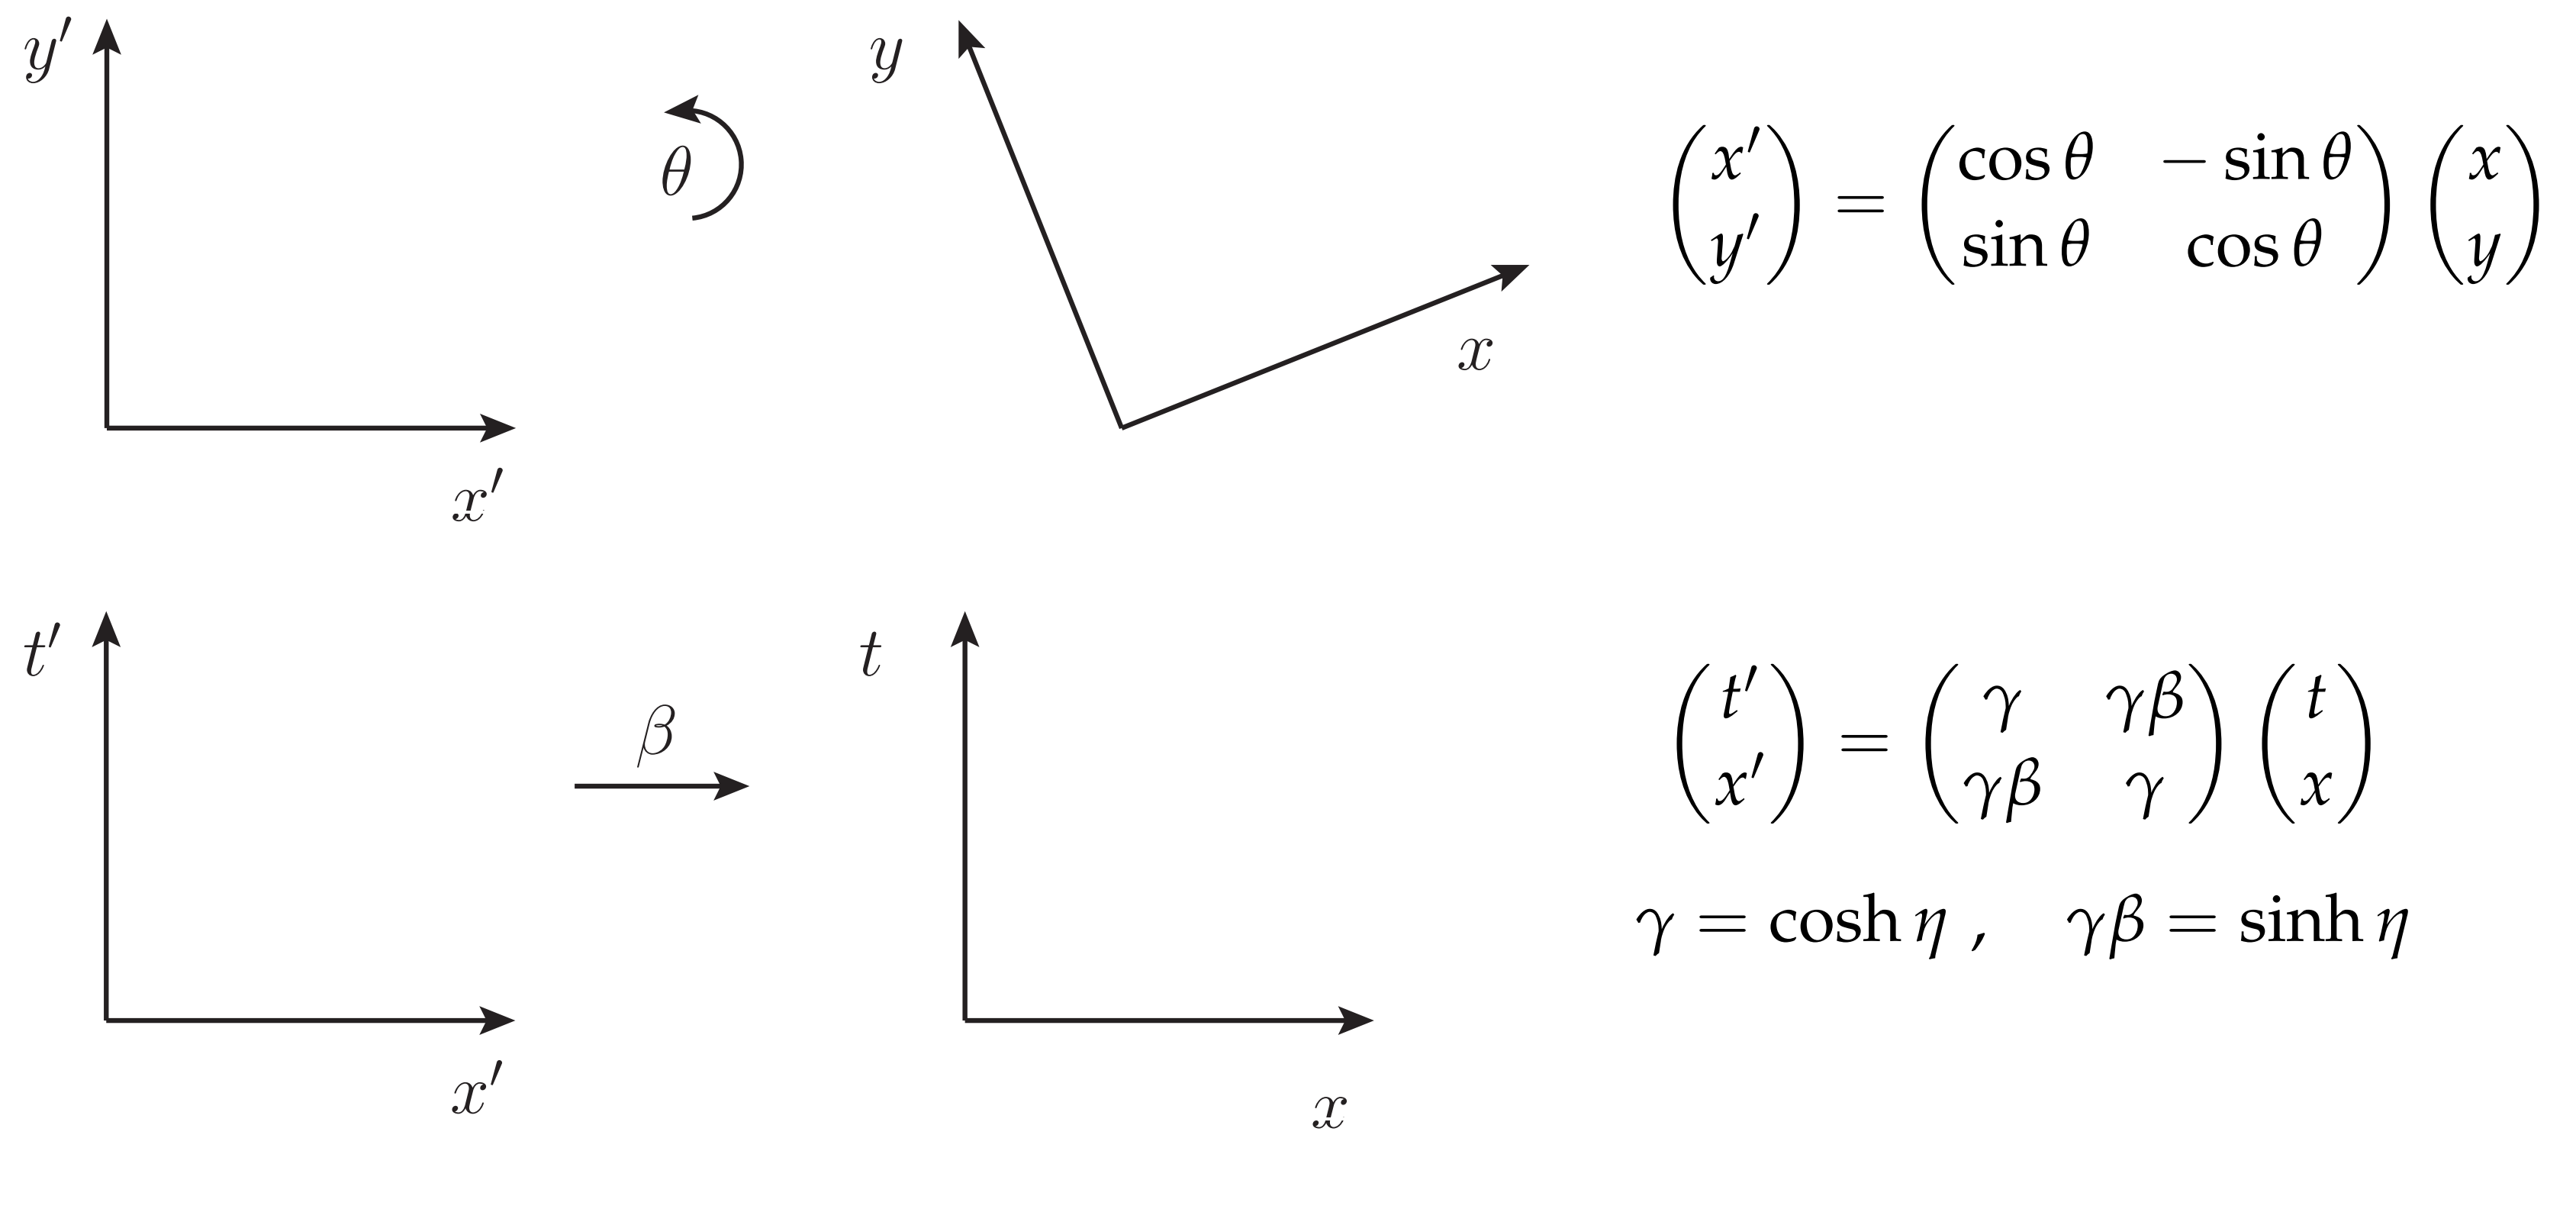
\includegraphics[scale=0.15]{Capitulos/Apendices/Ap_A3.png}
    \caption{Rotaciones y Boots}
%    \label{fig:my_label}
\end{figure}

Siguiendo la misma idea al grupo de rotaciones de $SO(3)$, algunos ejemplos de transformaciones de Lorentz. Por ejemplo las rotaciones al rededor de los ejes $x$, $y$ y $z$, son mediadas por las matrices:

\begin{equation}
    \left( \begin{array}{cccc}
    1 & 0 & 0 & 0 \\ 
    0 & 1 & 0 & 0 \\ 
    0 & 0 & \cos \theta _{x} & \sin \theta _{x} \\ 
    0 & 0 & -\sin \theta _{x} & \cos \theta _{x}
    \end{array} \right) ~,~\left( \begin{array}{cccc}
    1 & 0 & 0 & 0 \\ 
    0 & \cos \theta _{y} & 0 & -\sin \theta _{y} \\ 
    0 & 0 & 1 & 0 \\ 
    0 & \sin \theta _{y} & 0 & \cos \theta _{y}
    \end{array} \right) ~,~\left(  \begin{array}{cccc}
    1 & 0 & 0 & 0 \\ 
    0 & \cos \theta _{z} & \sin \theta _{z} & 0 \\ 
    0 & -\sin \theta _{z} & \cos \theta _{z} & 0 \\ 
    0 & 0 & 0 & 1
    \end{array}\right) ~.
    \label{rotaciones}
\end{equation}

También tenemos los boots en las direcciones $x$, $y$ y $z$

\begin{equation}
\left( 
\begin{array}{cccc}
\cosh \eta _{x} & \sinh \eta _{x} & 0 & 0 \\ 
\sinh \eta _{x} & \cosh \eta _{x} & 0 & 0 \\ 
0 & 0 & 1 & 0 \\ 
0 & 0 & 0 & 1
\end{array}
\right) ~,~\left( \begin{array}{cccc}
\cosh \eta _{y} & 0 & \sinh \eta _{y} & 0 \\ 
0 & 1 & 0 & 0 \\ 
\sinh \eta _{y} & 0 & \cosh \eta _{y} & 0 \\ 
0 & 0 & 0 & 1%
\end{array}
\right) ~,~\left( \begin{array}{cccc}
\cosh \eta _{z} & 0 & 0 & \sinh \eta _{z} \\ 
0 & 1 & 0 & 0 \\ 
0 & 0 & 1 & 0 \\ 
\sinh \eta _{z} & 0 & 0 & \cosh \eta _{z}
\end{array} \right) ~,
\label{boots}
\end{equation}
donde $\eta_{i}$ está relacionada con la velocidad $\beta_{i}=v_{i}$ del boost en la dirección $i$ por

\begin{equation*}
    \cosh \eta _{i}= \gamma_{i}=\frac{1}{\sqrt{1-v_{i}^{2}}}~,~\sinh \beta _{i}= \gamma_{i}\beta_{i} =\frac{v_{i}}{\sqrt{1-v_{i}^{2}}}~.
\end{equation*}
%~~\text{Aqui el doble índice no implica suma.}
Por otro lado, la reflexión total
\begin{equation}
\left( \begin{array}{cccc}
-1 & 0 & 0 & 0 \\ 
0 & -1 & 0 & 0 \\ 
0 & 0 & -1 & 0 \\ 
0 & 0 & 0 & -1
\end{array}\right)
~,
\end{equation}
 es también una transformación de Lorentz, así como lo es la inversión temporal
\begin{equation}
\left(\begin{array}{cccc}
-1 & 0 & 0 & 0 \\ 
0 & 1 & 0 & 0 \\ 
0 & 0 & 1 & 0 \\ 
0 & 0 & 0 & 1
\end{array}\right)~.
\end{equation}

La elección de los ejemplos que mostramos no es aleatoria: cualquier transformación de Lorentz puede descomponerse como un producto de estos cuatro tipos de transformaciones.\\

Las matrices de los ejemplos anteriores dan una representación del grupo de Lorentz sobre $\mathbb{C}^{4}$.\\
Aquí vamos a hacer un estudio más general de las representaciones del grupo de Lorentz y para ello estudiaremos su álgebra de Lie. Pero antes de eso, se hablará un poco acerca de la estructura de este grupo.

\subsubsection{Componentes del grupo de Lorentz}

Al tomar el determinante de ambos miembros de la ecuación (\ref{eqA31}) se obtiene:
\begin{equation}
    \det (\Lambda) = \pm 1~,
\end{equation}
esto define dos sub conjuntos de las transformaciones de Lorentz:
\begin{itemize}
    \item \textbf{Transformaciones Propias} si $\det (\Lambda) = +1$
    \item \textbf{Transformaciones Impropias} si $\det (\Lambda) = -1$
\end{itemize}

Ejemplos de transformaciones propias son: \emph{la identidad, las rotaciones, la reflexión total}. Mientras que la \emph{reflexión espacial} es un ejemplo de transformación impropia.\\

Hay una clasificación adicional dentro del grupo de Lorentz, que sale de escribir la componente $00$ de la ecuación (\ref{eqA31})

\begin{equation}
    (\Lambda^{0}_{0})^{2}-\sum_{j=1}^{3}(\Lambda^{j}_{0})^{2}=1~ \implies \qty(\Lambda^{0}_{~0})^{2} \geq 0 ~~\implies~\Lambda^{0}_{0} \geq 1 ~~ \text{ó} ~~ \Lambda^{0}_{0}  \leq -1~.
\end{equation}

\begin{minipage}[b]{0.7 \textwidth}
    El grupo de Lorentz consiste de cuatro componentes conexas (Ver figura \ref{Grupo de Lorentz}).\\

    \begin{itemize}
        \item [] $L_{+}^{\uparrow}$:  $\det \Lambda = + 1 ~~ \Lambda^{0}_{0} \geq 1$
        \item [] $L_{+}^{\downarrow}$:  $\det \Lambda = + 1 ~~ \Lambda^{0}_{0} \leq -1$
        \item [] $L_{-}^{\uparrow}$:  $\det \Lambda = - 1 ~~ \Lambda^{0}_{0} \geq 1$
        \item [] $L_{-}^{\uparrow}$:  $\det \Lambda = - 1 ~~ \Lambda^{0}_{0} \leq -1$
    \end{itemize}

\end{minipage}
\begin{minipage}[b]{0.3 \textwidth}
    \begin{figure}[H]
        \centering
        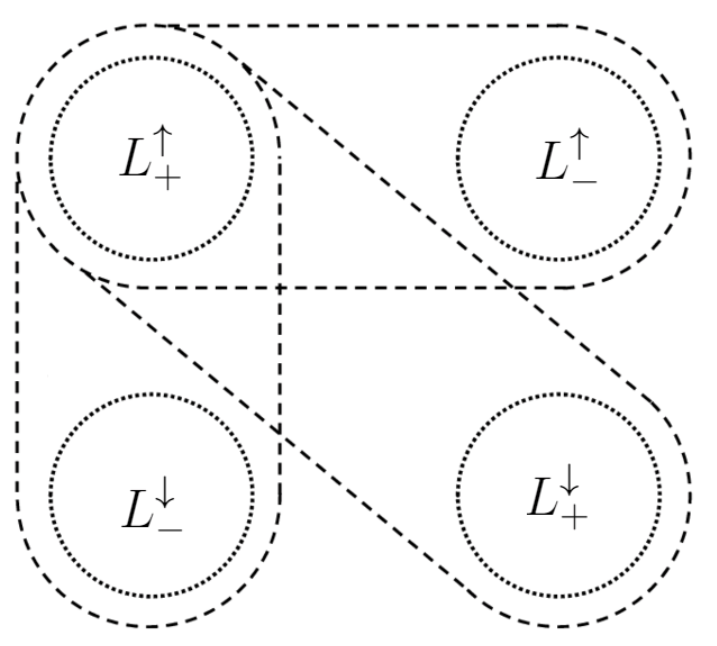
\includegraphics[width = 2.5cm]{Capitulos/Apendices/Ap_A.png}
        \caption{}
        \label{Grupo de Lorentz}
    \end{figure}
\end{minipage}

Las cuatro componentes conexas del grupo de Lorentz se esquematizan con círculos punteados en la figura, mientras que las líneas de trazos encierran a los tres subgrupos del grupo de Lorentz (note que todo grupo debe contener a $L_{+}^{\uparrow}$ ya que dicha componente es la que contiene a la identidad). El subgrupo $L_{+}^{\uparrow} \cup L_{+}^{\downarrow}$ se conoce como Grupo de Lorentz propio y se denota por $SO(3,1)$ y es el relevante para toda la fenomenología de partículas. (El $3$ por la dimensión espacial, el $1$ por la temporal). En detalle se tiene

\begin{enumerate}
    \item \textbf{Ortocronas} $(\Lambda^{0}_{0} \geq 1)$ \textbf{propias} ($\det \Lambda = + 1$)\\
    
    Forman grupo y es isomorfo a $SO(3,1)$. En adelante a $L_{+}^{\uparrow}$ lo llamaremos ``\emph{grupo de Lorentz propio ortocrono}''. Sus elementos son transformaciones continuas (grupo de Lie) que se pueden conectar con la identidad mediante sucesivas transformaciones infinitesimales. Sus elementos son rotaciones en las tres dimensiones espaciales y boosts (transformaciones de Lorentz puras). Estas últimas relacionan los sistemas de coordenadas de dos observadores inerciales (que se mueven con velocidad relativa constante).\\

    Las demás transformaciones obviamente no forman grupo y se pueden escribir como producto de inversiones (transformaciones discretas) y transformaciones de Lorentz ortocronas propias $\Lambda_{P}$. Estas son:
    \vspace{1cm}
    \item \textbf{No ortocronas} ($\Lambda^{0}_{0} \leq -1$) \textbf{propias} ($\det \Lambda = + 1$)   \\

    Transformaciones tipo $\Lambda_{P} \times \qty{\text{diag} \qty(-,-,-,-),~ \text{diag} \qty(-,-,+,+),~ \text{diag} \qty(-,+,-,+),~ \text{diag} \qty(-,+,+,-)}$. Incluye a las inversiones totales, $\text{diag} (-,-,-,-)$.
   \vspace{1cm} 
   \item  \textbf{Ortocronas} $(\Lambda^{0}_{0} \geq 1)$ \textbf{impropias} ($\det \Lambda = - 1$)\\

   Transformaciones tipo $\Lambda_{P} \times \qty{\text{diag} \qty(+,+,+,-),~ \text{diag} \qty(+,+,-,+),~ \text{diag} \qty(+,-,+,+),~ \text{diag} \qty(+,-,-,-)}$. Incluye a las inversiones espaciales, $\text{diag} (+,-,-,-)$.
   \vspace{1cm} 
   \item \textbf{No ortocronas} ($\Lambda^{0}_{0} \leq -1$) \textbf{impropias} ($\det \Lambda = - 1$)   \\
   Transformaciones tipo $\Lambda_{P} \times \qty{\text{diag} \qty(-,-,-,+),~ \text{diag} \qty(-,-,+,-),~ \text{diag} \qty(-,+,-,-),~ \text{diag} \qty(-,+,+,+)}$. Incluye a las inversiones temporales, $\text{diag} (-,+,+,+)$.
\end{enumerate}


%El subgrupo $L_{+}^{\uparrow}$ se conoce como \emph{Grupo de Lorentz propio ortócrono}. Sin embargo, este no es el único subgrupo de grupo de Lorentz. De hecho, $L_{+}^{\uparrow}$ junto a cualquiera de las otras tres componentes son subgrupos. El que también nos va a interesar $L_{+}^{\uparrow} \cup L_{+}^{\downarrow}$, que se conoce como Grupo de Lorentz propio, se denota por $SO(3,1)$ y es el relevante para toda la fenomenología de partículas. (El $3$ por la dimensión espacial, el $1$ por la temporal).\\

\vspace{0.4cm}
Observe que si queremos ver cuantos parámetros tiene el grupo de Lorentz (de transformaciones ortocronas propias), consideramos una transformación infinitesimal arbitraria 
\begin{equation}
    \Lambda^{\mu}_{~\nu}=\delta^{\mu}_{\nu}+\omega^{\mu}_{~\nu}
\end{equation}
donde (\ref{eqA31}) implica que $\omega_{\mu \nu}=-\omega_{\nu \mu}$.\\

Siendo $\omega$ antisimétrica tiene solamente 6 parámetros independientes, lo que en efecto garantiza que cualquier $\Lambda$ puede escribirse como producto de rotaciones $(R)$ Parametrizadas con 3 ángulos $\theta \in [0,2\pi]$ (ver eq. \ref{rotaciones}), y boots $(L)$ que se parametrizan especificando las tres componentes de la velocidad $\beta \in [-1,1]$ (ó $\eta \in [-\infty,\infty]$) a lo largo de $x$, $y$ o $z$ (ver eq. \ref{boots}).  



\subsection{Álgebra del grupo de Lorentz}

En esta sección, vamos a encontrar los generadores de las rotaciones y los boosts, y los conmutadores entre dichos generadores. Como las relaciones de conmutación valen lo mismo en cualquier representación (recuerde por ejemplo lo que vimos sobre las representaciones de $su(2)$) al hacer esto vamos a tener determinada en forma abstracta el álgebra del grupo de Lorentz. Una vez que se tenga el álgebra, será cuestión de estudiar sus representaciones para ver las que se inducen sobre el grupo.\\

A modo de ejemplo, calculemos el generador de los boots en la dirección $x$. Recuerde que dichos boots se representan por la siguiente matriz:

\begin{equation}
\Lambda \left( \eta _{x}\right) =\left( 
\begin{array}{cccc}
\cosh \eta _{x} & \sinh \eta _{x} & 0 & 0 \\ 
\sinh \eta _{x} & \cosh \eta _{x} & 0 & 0 \\ 
0 & 0 & 1 & 0 \\ 
0 & 0 & 0 & 1
\end{array}
\right)~. 
\end{equation}

Ahora, buscamos una matriz $M_{tx}=-M_{xt}$ tal que resulte
\begin{equation}
    \Lambda \qty(\eta_{x}) = e ^ {\frac{i}{2} \qty(\eta_{x}M^{tx}-\eta_{x}M^{xt})}  = e^{i\eta_{x}M^{tx}}~.
    \label{eqA_42}
\end{equation}

Aquí $\eta_{x}$ juega el rol análogo de los $\omega^{IJ}$ de la ecuación (\ref{A8}). Por ese motivo $M_{xt}$ aparece multiplicado por $-\eta_{x}$, que recuerde que $\omega^{IJ}=\omega^{JI}$. Agregamos además la unidad imaginaria $i$ para ser consistentes con la definición más común de los generadores que suele hacerse en la literatura de física. En virtud de la ecuación (\ref{eqA_42}) se tiene que cumplir que 
\begin{equation}
    M^{tx} = -i \eval{\dv{\Lambda (\eta_{x})}{\eta_{x}}}_{\eta_{x} = 0}~, 
\end{equation}
que introduciendo la forma explicita de boost nos da
\begin{equation}
\begin{split}
    M^{tx} &= -i \eval{\dv{\Lambda (\beta_{x})}{\beta_{x}}}_{\beta_{x} = 0} \\
    &= -i\left(  \begin{array}{cccc}
    0 & 1 & 0 & 0 \\ 
    1 & 0 & 0 & 0 \\ 
    0 & 0 & 0 & 0 \\ 
    0 & 0 & 0 & 0 
    \end{array} \right) ~.
\end{split}
\end{equation}

Siguiendo un proceso similar se puede obtener los generadores asociados a los boots en $y$ t $z$:
\begin{equation}
    M^{ty}=-i\left(  \begin{array}{cccc} 
    0 & 0 & 1 & 0 \\ 
    0 & 0 & 0 & 0 \\ 
    1 & 0 & 0 & 0 \\ 
    0 & 0 & 0 & 0 
    \end{array} \right) ~,~\ M^{tz}=-i\left( \begin{array}{cccc}
    0 & 0 & 0 & 1 \\ 
    0 & 0 & 0 & 0 \\ 
    0 & 0 & 0 & 0 \\ 
    1 & 0 & 0 & 0
    \end{array}
\right) ~,
\end{equation}
 y los asociados a las rotaciones en $x$, $y$ y $z$

 \begin{equation}
M^{yz}=-i\left( 
\begin{array}{cccc}
0 & 0 & 0 & 0 \\ 
0 & 0 & 0 & 0 \\ 
0 & 0 & 0 & 1 \\ 
0 & 0 & -1 & 0
\end{array}
\right) ~,~\ M^{zx}=-i\left( 
\begin{array}{cccc}
0 & 0 & 0 & 0 \\ 
0 & 0 & 0 & -1 \\ 
0 & 0 & 0 & 0 \\ 
0 & 1 & 0 & 0
\end{array}
\right) ~,~\ M^{xy}=-i\left( 
\begin{array}{cccc}
0 & 0 & 0 & 0 \\ 
0 & 0 & 1 & 0 \\ 
0 & -1 & 0 & 0 \\ 
0 & 0 & 0 & 0
\end{array}
\right) ~.
\end{equation}

Note que, salvo por la dimensión y por el factor $-i$ asociado al cambio de definición, los generadores de las rotaciones tienen la misma forma ya encontradas en las ecuaciones (\ref{eqA_18}) y (\ref{eqA_19}). Puede corroborarse que se cumple:
\begin{equation}
    \comm{M^{\mu \nu}}{M^{\rho \sigma}} = i \qty(g^{\mu \sigma}M^{\nu \rho} + g^{\nu \rho}M^{\mu \sigma} - g^{\mu \rho}M^{\nu \sigma}-g^{\nu \sigma}M^{\mu \rho} )~,
    \label{alorentz}
\end{equation}
haciendo los conmutadores entre las matrices (No olvide que los subíndices aquí etiquetan a las matrices y no denotan componentes). Esta es el álgebra del grupo de Lorentz propio y se denota por $so(3,1)$.\\

Tenga presenta también que, como la variedad paramétrica de los boots no es compacta, sus generadores no son hermíticos. Ya con el álgebra de Lorentz, se analizará unos desarrollos que nos permitirán escribir las representaciones de $so(3,1)$ en términos de representaciones de $su(2)$. Para ello primero, veamos una forma de reescribir las relaciones entre los generadores $M_{\mu \nu}$ que definen el álgebra de Lorentz. Definimos

\begin{eqnarray}
J^{i} &\equiv &\frac{1}{2}\epsilon ^{ijk}M^{jk}~\Longrightarrow ~\left\{ 
\begin{array}{c}
J^{1}=M^{23}=-M^{32} \\ 
J^{2}=M^{31}=-M^{13} \\ 
J^{3}=M^{12}=-M^{21}
\end{array}
\label{eqA_1.36}
\right.  \\
K^{i} &\equiv &M^{i0}=-M^{0i}
\label{eqA_1.37}
\end{eqnarray}

%\begin{equation}
%    J_{i} \equiv \frac{1}{2} \epsilon_{ijk} M_{jk}~,
%    K_{i} \equiv M_{i0}~,
%\end{equation}
donde $i,j,k$ hacen referencia a la parte espacial. Así:

\begin{eqnarray}
J^{1} &=&\left( 
\begin{array}{cccc}
0 & 0 & 0 & 0 \\ 
0 & 0 & 0 & 0 \\ 
0 & 0 & 0 & -i \\ 
0 & 0 & i & 0%
\end{array}%
\right) ~\ ,~\ \ J^{2}=\left( 
\begin{array}{cccc}
0 & 0 & 0 & 0 \\ 
0 & 0 & 0 & i \\ 
0 & 0 & 0 & 0 \\ 
0 & -i & 0 & 0%
\end{array}%
\right) ~\ ,~\ \ J^{3}=\left( 
\begin{array}{cccc}
0 & 0 & 0 & 0 \\ 
0 & 0 & -i & 0 \\ 
0 & i & 0 & 0 \\ 
0 & 0 & 0 & 0%
\end{array}%
\right)  \\
K^{1} &=&\left( 
\begin{array}{cccc}
0 & i & 0 & 0 \\ 
i & 0 & 0 & 0 \\ 
0 & 0 & 0 & 0 \\ 
0 & 0 & 0 & 0%
\end{array}%
\right) ~\ ,~\ K^{2}=\left( 
\begin{array}{cccc}
0 & i & 0 & 0 \\ 
i & 0 & 0 & 0 \\ 
0 & 0 & 0 & 0 \\ 
0 & 0 & 0 & 0%
\end{array}%
\right) ~\ ,~\ K^{3}=\left( 
\begin{array}{cccc}
0 & 0 & 0 & i \\ 
0 & 0 & 0 & 0 \\ 
0 & 0 & 0 & 0 \\ 
i & 0 & 0 & 0%
\end{array}%
\right) 
\end{eqnarray}

Es bien conocido que los generadores de las rotaciones cumplen que 
\begin{equation}
    \comm{J^{i}}{J^{j}} = i \epsilon^{ijk}J^{k}~,
\end{equation}
indicándonos que el álgebra asociada al grupo de rotaciones es $su(2)$. Veamos ahora los otros conmutadores, comenzando por el de dos boost:

\begin{eqnarray*}
\left[ K^{i},K^{j}\right]  &=&\left[ M^{i0},M^{j0}\right]  \\
&=&i\left( g^{i0}M^{0j}+g^{oj}M^{io}-g^{ij}M^{00}-g^{00}M^{ij}\right)  \\
&=&i\left( -g^{00}M^{ij}\right) .
\end{eqnarray*}

Usando que $M^{ij}=-M^{ji}$, se puede reescribir $M^{ij}$ como $\left(M^{ij}-M^{ji}\right) /2$. Entonces

\begin{equation}
\left[ K^{i},K^{j}\right] =-i\left[ \frac{1}{2}\left( M^{ij}-M^{ji}\right) 
\right] =-i\epsilon ^{kij}J^{k}
\end{equation}

donde se ha usado que $J_{k}\epsilon _{kmn}=\frac{1}{2}\left(M_{mn}-M_{nm}\right) $, relaci\'{o}n que se puede probar empleando la propiedad $\epsilon _{ijk}\epsilon _{imn}=\delta _{jm}\delta _{kn}-\delta_{jn}\delta _{km}$. Vemos entonces que los generadores de boost no conmutan entre si. De forma análoga se puede calcular el conmutador restante entre generadores de boost y rotaciones. En resumen se tiene que el álgebra de lie es:

\begin{equation}
    \comm{J^{i}}{J^{j}}=i\epsilon^{ijk}J^{k}~,~~\comm{K^{i}}{K^{j}}=-i\epsilon^{ijk}J^{k}~,~~\comm{J^{i}}{K^{j}}=i\epsilon^{ijk}K^{k}   ~.     
\end{equation}

Note que las relaciones anteriores permiten concluir que los boost no forman un grupo ya que el álgebra de sus generadores no es cerrada, a diferencia de lo que sucede con las rotaciones.\\

Conviene ahora definir:
\begin{equation}
    \bar{A}\equiv \frac{1}{2} \qty(\bar{J}-i\bar{K})~,~~ \bar{B}\equiv \frac{1}{2} \qty(\bar{J}+i\bar{K})~,
\end{equation}
siendo $\bar{J}=(J^{1},J^{2},J^{3})$ y $\bar{K}=(K^{1},K^{2},K^{3})$, el álgebra de Lorentz es ahora una suma directa de dos $su(2)$. Para ver esto, hallemos los conmutadores entre estos nuevos generadores

\begin{eqnarray}
\left[ A^{i},A^{j}\right]  &=&\left[ \frac{1}{2}\left( J^{i}-iK^{i}\right) ,
\frac{1}{2}\left( J^{j}-iK^{j}\right) \right]   \notag \\
&=&\frac{1}{4}\left( \left[ J^{i},J^{j}\right] -i\left[ K^{i},J^{j}\right] -i
\left[ J^{i},K^{j}\right] -\left[ K^{i},K^{j}\right] \right)   \notag \\
&=&\frac{1}{4}\left( i\epsilon ^{ijk}J^{k}+\epsilon ^{ijk}K^{k}+\epsilon
^{ijk}K^{k}+i\epsilon ^{ijk}J^{k}\right) =\frac{i\epsilon ^{ijk}}{2}\left(
J^{k}-iK^{k}\right)   \notag \\
&=&i\epsilon ^{ijk}A^{k}~.
\end{eqnarray}%
\begin{eqnarray}
\left[ B^{i},B^{j}\right]  &=&\left[ \frac{1}{2}\left( J^{i}+iK^{i}\right) ,
\frac{1}{2}\left( J^{j}+iK^{j}\right) \right]   \notag \\
&=&\frac{1}{4}\left( \left[ J^{i},J^{j}\right] +i\left[ J^{i},K^{j}\right] +i
\left[ K^{i},J^{j}\right] -\left[ K^{i},K^{j}\right] \right)   \notag \\
&=&\frac{1}{4}\left( i\epsilon ^{ijk}J^{k}-\epsilon ^{ijk}K^{k}-\epsilon
^{ijk}K^{k}+i\epsilon ^{ijk}J^{k}\right) =\frac{i\epsilon ^{ijk}}{2}\left(
J^{k}+iK^{k}\right)   \notag \\
&=&i\epsilon ^{ijk}B^{k}~.
\end{eqnarray}

\begin{eqnarray}
\left[ A^{i},B^{j}\right]  &=&\left[ \frac{1}{2}\left( J^{i}-iK^{i}\right) ,
\frac{1}{2}\left( J^{j}+iK^{j}\right) \right]   \notag \\
&=&\frac{1}{4}\left( \left[ J^{i},J^{j}\right] +i\left[ J^{i},K^{j}\right] -i
\left[ K^{i},J^{j}\right] +\left[ K^{i},K^{j}\right] \right)   \notag \\
&=&\frac{1}{4}\left( i\epsilon ^{ijk}J^{k}-\epsilon ^{ijk}K^{k}+\epsilon
^{ijk}K^{k}-i\epsilon ^{ijk}J^{k}\right)   \notag \\
&=&0~.
\end{eqnarray}

Vemos entonces que los operadores $A_{i}$ y $B_{i}$ conmutan entre ellos, es decir sus álgebras son independientes entre sí, y además, el álgebra de cada uno de ellos es el álgebra $su(2)$. En términos matemáticos, $so(3,1) = su(2) \oplus su(2)$ y es localmente isomorfo a $SU(2)\times SU(2)$ por tener la misma álgebra. De esta propiedad para el álgebra de Lie correspondiente al grupo de Lorentz se desprende que 

\begin{cabox}
    Las representaciones Lorentz irreducibles se puedan etiquetar por el par de semi-enteros $(j_{1},j_{2})$ de dimensión $(2j_{1}+1)(2j_{2}+1)$, que corresponden al espín de la representación de cada $su(2)$.
\end{cabox}

Notese que hemos encontrado irreps del grupo de Lorentz de dimensión finita, pero no son unitarias porque no es compacto.

%--------------------------------
otra forma de escribir los generadores del grupo de Lorentz es la siguiente. Tomamos como parámetros los $6$ elementos independientes de una matriz antisimétrica $\omega_{\mu \nu}=-\omega_{\nu \mu}$. Los generadores son entonces las $6$ componentes independientes del operador antisimétrico $M^{\mu \nu}=-M^{\nu \mu}$,
\begin{equation}
    \Lambda = e^{-\frac{i}{2}\omega_{\mu\nu}M^{\mu \nu}}~,
    \label{eqA1_2.19}
\end{equation}
(el factor $1/2$ compensa el hecho que sumaos sobre $\mu,\nu$). Al definir $\theta$ y $\eta$ mediante
\begin{eqnarray}
\theta ^{k} &=&\frac{1}{2}\epsilon ^{klm}\omega ^{lm}~\Rightarrow ~\left\{ 
\begin{array}{c}
\theta ^{1}=\omega ^{23}=-\omega ^{32}=\omega _{23}=-\omega _{32} \\ 
\theta ^{2}=\omega ^{31}=-\omega ^{13}=\omega _{31}=-\omega _{13} \\ 
\theta ^{3}=\omega ^{12}=-\omega ^{21}=\omega _{12}=-\omega _{21}
\end{array}
\right.  \\
\eta ^{k} &=&\omega ^{0k}=-\omega ^{k0}=-\omega _{0k}=\omega _{k0}
\end{eqnarray}
tenemos que,
\begin{equation}
\begin{split}
    \frac{1}{2}\omega_{\mu \nu}M^{\mu \nu} &=  \omega_{12}M^{12}+\omega_{31}M^{31}+\omega_{23}M^{23}+\omega_{i0}M^{i0} \\
    & = \theta^{i}J^{i} + \eta^{i}K^{i}  \\
    & \equiv \vb*{\theta} \cdot \vb{J} + \vb*{\eta} \cdot \vb{K}~,  
\end{split}
\end{equation}
por lo que
\begin{equation}
    \Lambda=\ee^{-i\qty(\vb*{\theta} \cdot \vb{J} + \vb*{\eta} \cdot \vb{K}) }~,
    \label{eqA_71}
\end{equation}
Observe que 
\begin{equation}
    \Lambda^{-1}=\ee^{i\qty(\vb*{\theta} \cdot \vb{J} + \vb*{\eta} \cdot \vb{K}) } \neq \Lambda^{\dagger}=\ee^{i\qty(\vb*{\theta} \cdot \vb{J} - \vb*{\eta} \cdot \vb{K}) }
\end{equation}

lo que quiere decir que las irreps del grupo de Lorentz de dimensión finita no son unitarias, porque no es compacto. Al redefinir $M^{\mu \nu}\equiv J^{\mu \nu}$, se tiene que su representación es una matriz $4\times 4$ $(J^{\mu \nu})^{\rho}_{~\sigma}$.\\

La forma explicita de estos generadores es

\begin{equation}
    (J^{\mu \nu})^{\rho}_{~\sigma} = i \qty(g^{\mu \rho} \delta^{\nu}_{~\sigma}-g^{\nu \rho} \delta^{\mu}_{~\sigma})~,
    \label{eqA2.32}
\end{equation}
  los cuales satisfacen el álgebra de Lie dada en (\ref{eq_A106})-

\subsection{Representaciones Tensoriales}

Lo que acabamos de ver es la representación en cuatro dimensiones del grupo de Lorentz, que nos ha servido para definir el grupo. Podemos plantearnos si es irreducible (lo es) y si es su representación no trivial de dimensión más pequeña (veremos que no lo es). Se llama representación vectorial del grupo de Lorentz:

\begin{equation}
    \Lambda^{\mu}_{~\nu}=\qty\bigg[e^{-i\qty(\vb*{\theta} \cdot \vb{J} + \vb*{\eta} \cdot \vb{K}) }]^{\mu}_{~\nu}=~\qty\bigg[e^{-i\qty(\frac{1}{2} \omega_{\alpha \beta}J^{\alpha \beta})}]^{\mu}_{~\nu},
\end{equation}

Un cuadrivector contravariante $V^{\mu}$ (ó covariante $V_{\mu}$) es un vector que pertenece a un espacio vectorial invariante e irreducible que se transforma como
\begin{equation}
    V^{\mu \prime}=\Lambda^{\mu}_{~\nu} V^{\nu}~~,~~V_{\mu \prime}=\Lambda_{\mu}^{~\nu} V_{\nu}~,
 \end{equation}
 donde $\Lambda^{\mu}_{~\nu}$ y $\Lambda_{\mu}^{~\nu}$ son representaciones equivalentes, dado que están relacionadas mediante una transformación de semejanza $S=g_{\mu \nu}$ tal que $\Lambda^{\mu}_{~\nu}=g^{\mu \rho}\Lambda_{\rho}^{~\sigma}g_{\sigma \nu}$.\\

 Se debe tener en cuenta que el término representación se asocia con el espacio de representación. Así diremos que $V^{\mu}$ y $V_{\mu}$ son irreps equivalentes. $V_{\mu}$ es el vector asociado a $V^{\mu}$ en el espacio dual, así que la matriz $\Lambda_{\mu}^{~\nu}$ es la inversa de $\Lambda^{\mu}_{~\nu}$, dado que de ((\ref{eqA31}): $g_{\mu \nu }=\Lambda _{~\mu }^{\alpha }\Lambda _{~\nu }^{\beta}g_{\alpha \beta }$)
 
\begin{eqnarray*}
g_{\alpha \beta }\Lambda _{~\mu }^{\alpha }\Lambda _{~\nu }^{\beta }
&=&\Lambda _{\beta \mu }\Lambda _{~\nu }^{\beta }=g_{\mu \nu }, \\
g_{\alpha \beta }\Lambda _{~\mu }^{\alpha }\Lambda _{~\nu }^{\beta }
&=&\Lambda _{~\mu }^{\alpha }\Lambda _{\alpha \nu }=g_{\mu \nu },
\end{eqnarray*}%
y multiplicando la primera linea anterior por $g^{\tau \mu }$%
\begin{eqnarray}
g^{\tau \mu }\Lambda _{\beta \mu }\Lambda _{~\nu }^{\beta } &=&g^{\tau \mu
}g_{\mu \nu }~\Longrightarrow ~\Lambda _{\beta }^{~\tau }\Lambda _{~\nu
}^{\beta }=g^{\tau \mu }g_{\mu \nu }=g_{~\nu }^{\tau }~,  \notag \\
&\therefore &~\Lambda _{\beta }^{~\mu }\Lambda _{~\nu }^{\beta }=g_{~\nu
}^{\mu }=\delta _{\nu }^{\mu }~.
\end{eqnarray}
 
Se pueden construir representaciones de dimensiones mayores mediante el producto tensorial. A estas representaciones se llaman tensoriales y sus vectores son tensores con varios índices (Su número se llama rango). Así, un tensor $T^{\mu \nu}$ on dos índices contravariantes es un objeto que transforma bajo Lorentz como:
\begin{equation}
    T^{\mu \nu} = \Lambda^{\mu}_{~\mu^{\prime}} \Lambda^{\nu}_{~\nu^{\prime}} T^{\mu^{\prime} \nu^{\prime}}~.
\label{eqA2.34}
\end{equation}

En general, un tensor con índices arriba transforma con $\Lambda^{\mu}_{~\nu}$, y con índices abajo transforma con $\Lambda_{\mu}^{~\nu}$.\\

Los tensores son ejemplos de representaciones del grupo de Lorentz, por ejemplo $T^{\mu}_{~\nu}$ con dos índices contravariantes tiene $4^{2}=16$ componentes, las cuales constituyen la base para una representación en dimensión 16. Sin embargo, esta representación es reducible, dado que de la ecuación (\ref{eqA2.34}) se observa que, si $T^{\mu}_{~\nu}$ es antisimétrico, después de una transformación de Lorentz permanece antisimétrico, al igual que si es simétrico entonces permanece simétrico. Esto quiere decir que las partes simétrica y antisimétrica del tensor no se mezclan y por tanto la representación en 16 dimensiones es reducible a una rep. de 6 dimensiones antisimétrica $A^{\mu \nu}=(1/2)(T^{\mu \nu}-T^{\nu \mu})$, y una rep. de 10 dimensiones simétrica $S^{\mu \nu}=(1/2)(T^{\mu \nu}+T^{\nu \mu})$.

La traza de un tensor se define como 
\begin{equation}
    S \equiv S^{\mu}_{~\mu}=g_{\mu \nu}S^{\mu \nu} ~~\implies~~ S^{\prime}=S^{ \prime \mu}_{~\mu}=\Lambda^{\mu}_{~\rho}\Lambda_{\mu}^{~\sigma} S^{\rho}_{~\sigma}=\delta^{\sigma}_{\rho}S^{\rho}_{~\sigma} = S^{\rho}_{~\rho}=S~,
\end{equation}
 lo que demuestra que la traza de un tensor permanente invariante ante transformaciones de Lorentz. Por lo tanto, si se tiene un tensor sin traza, este permanecerá sin traza luego de una T.L. y por ende, la representación simétrica de 10 dimensiones se descompone aún más en una representación sin traza simétrica irreducible de dimensión 9, $S^{\mu \nu}-(1/4)g^{\mu \nu}S$ y la representación unidimensional (escalar) $S$. Este hecho verifica que un tensor de segundo orden pueda escribirse como una suma directa de representaciones irreducibles
 \begin{equation}
     \vb*{4} \otimes \vb*{4} = \vb*{1} \oplus \vb*{6} \oplus \vb*{9}~,
 \end{equation}
donde la representación irreducible es denotada por su dimensionalidad en negrita. Por lo tanto $\vb*{1}$ es la rep. escalar (Unidimensional), $\vb*{4}$ la rep. de un cuadrivector, $\vb*{6}$ el tensor antisimétrico y $\vb*{9}$ el tensor simétrico sin traza. De este modo cualquier tensor arbitrario se escribe como:
\begin{equation}
\begin{split}
    T^{\mu \nu} &= \frac{1}{2}g^{ \mu \nu}T+A^{\mu \nu} + S^{ \mu \nu}~,  \text{donde}\\
    T =& T^{\mu}_{~\mu}\\
    A^{\mu \nu} &=\frac{1}{2}\qty(T^{\mu \nu} - T^{\nu \mu})\\
    S^{\mu \nu} &=\frac{1}{2}\qty(T^{\mu \nu} + T^{\nu \mu})-\frac{1}{4}g^{\mu \nu}T
\end{split}
\end{equation}
 Por este mismo razonamiento, $T^{\mu}_{~\nu}$, $T_{\mu}^{~\nu}$ y $T_{\mu \nu}$ son representaciones (reducibles) equivalentes del grupo de Lorentz.\\

 Es interesante ver ver como se transforman las irrepsdel grupo de Lorentz bajo el sub grupo de las rotaciones.\\
 Como sabemos el comportamiento de un tensor bajo una transformación genérica de Lorentz, conocemos en particular sus propiedades de transformación bajo el subgrupo de rotación $SO(3)$, y por lo tanto nos podemos preguntar cuál es el momento angular $j$ de las diversas representaciones de tensor. Recuerde que las representaciones de $SO(3)$ están etiquetadas por un índice $j$ que toma valores enteros $j=1,2,\ldots,$ y la dimensión de la representación etiquetada por $j$ es $2j + 1$. Dentro de cada representación, estos $2j + 1$ estados están etiquetados por $j_{z}=-j,\ldots,j$. Para $SO(3)$, es más común denotar la representación como $\vb*{j}$, es decir, etiquetarla con el momento angular en lugar de con la dimensión de la representación, $2j+1$. En esta notación, $\vb*{0}$ es el escalar (también llamado el singlete), $\vb*{1}$ es un triplete con componentes $j_{z}=-1,0,1$, dimensión 5,... etc. (si preferimos usar la misma convención que en el caso del grupo de Lorentz, es decir, los etiquetamos por su dimensionalidad, deberíamos escribir $\vb*{1}$, $\vb*{3}$, $\vb*{5}$,...).\\

 Un escalar de Lorentz, por supuesto, también es escalar bajo rotaciones, por lo que tiene $j=0$. Un cuadrivector $V^{\mu}=(V^{0},\vb*{V})$ es una representación irreducible del grupo de Lorentz, ya que una transformación de Lorentz genérica mezcla los cuatro componentes, pero desde el punto de vista del subgrupo $SO(3)$ es reducible: las rotaciones espaciales no mezclan $V^{0}$ con $\vb*{V}$, por ende $V^{0}$ es invariante bajo rotaciones espaciales, por lo que tiene asociado espín $j = 0$, mientras que los tres componentes espaciales $V^{i}$ forman una representación tridimensional irreducible de $SO(3)$, por lo que tienen espín $j = 1$. En el lenguaje de la teoría de grupos decimos que, desde el punto de vista de las rotaciones espaciales, un cuadrivector se puede descomponer en la suma directa de un escalar y una representación $j = 1$,\\
 \begin{equation}
     V^{\mu} \in \vb*{0}\oplus \vb*{1} ~~ \text{etiquetadas por $j=0,1$ bajo el grupo de rotaciones}.
 \end{equation}

 Ahora queremos entender qué momentos angulares aparecen en un tensor genérico $T^{\mu \nu}$ con dos índices. Por definición, un tensor $T^{\mu \nu}$ se transforma como el producto tensorial de dos representaciones de cuadrivectores. Entonces desde el punto de vista del grupo de rotaciones $SO(3)$
 \begin{equation}
 \begin{split}
     T^{\mu \nu} \in \vb*{4} \otimes \vb*{4} &= \vb*{1} \oplus \vb*{6} \oplus \vb*{9} \\
     &= (\vb*{0} \oplus \vb*{1}) \otimes (\vb*{0} \oplus \vb*{1})\\
     &= (\vb*{0} \otimes \vb*{0}) \oplus (\vb*{0} \otimes \vb*{1}) \oplus (\vb*{1} \otimes \vb*{0}) \oplus (\vb*{1} \otimes \vb*{1})\\
     &= \vb*{0} \oplus \vb*{1} \oplus \vb*{1} \oplus ( \vb*{0} \oplus \vb*{1} \oplus \vb*{2} ) ~.
 \end{split} 
 \end{equation}

donde se ha usado que el producto directo de irreps del grupo de las rotaciones obedece la regla de adición de momento angular estableciendo que al componer dos momentos angulares,

\begin{equation}
    j_{1} \otimes j_{2} = \abs{j_{1}-j_{2}} \oplus \abs{j_{1}-j_{2}}+1 \oplus  \cdots  \oplus \cdots j_{1}+j_{2}-1  \oplus j_{1}+j_{2}~.
\end{equation}

Así, en la descomposición de un tensor arbitrario $T^{\mu \nu}$ en representaciones del grupo de rotación, corresponde a la suma directa de las irreps asociadas a $j = 0$ (aparece dos veces), $j = 1$ (aparece tres veces) y la $j = 2$ una vez. Explícitamente

\begin{eqnarray*}
\mathbf{1} &:&~~\ T\in ~\mathbf{0~~\ \ }~\text{(Es tambi\'{e}n un escalar bajo rotaciones)}  \notag \\
\mathbf{6} &:&~~\ A^{\mu \nu }\in ~\mathbf{1\oplus 1}~\ \mapsto ~\left\{ 
\begin{array}{c}
A^{0i} \\ 
\frac{1}{2}\epsilon ^{ijk}A^{jk}%
\end{array}%
\right. \text{ \ \ (Corresponde a dos 3-vectores independientes bajo
rotaciones.)} \\
\mathbf{9} &:&~~\ S^{\mu \nu }\in ~\mathbf{0\oplus 1\oplus 2}~\ \mapsto
~\left\{ 
\begin{array}{c}
S^{00} \\ 
S^{0i} \\ 
S^{ij}~\ \ ;~\ \sum\limits_{i}S^{ij}=-S^{00}
\end{array}
\right.   \notag
\end{eqnarray*}

En general, un tensor $T^{\mu \nu \rho \ldots} $ con $N$ componentes contiene espines $j=0,1,\ldots,N.$

Como curiosidad, un tensor completamente antisimétrico de orden $4$, $A^{\mu \nu \rho \sigma}$, solo tiene una componente diferente de cero $A^{0123}$, de modo que se puede escribir como $A^{\mu \nu \rho \sigma} = a\epsilon^{\mu \nu \rho \sigma}$, por lo tanto es un escalar de Lorentz pues

\begin{equation}
    \epsilon^{\mu \nu \rho \sigma} = \Lambda^{\mu}_{~\mu^{\prime}} \Lambda^{\nu}_{~\nu^{\prime}} \Lambda^{\rho}_{~\rho^{\prime}} \Lambda^{\sigma}_{~\sigma^{\prime}} \epsilon^{\mu^{\prime} \nu^{\prime} \rho^{\prime} \sigma^{\prime}}=\det(\Lambda)\epsilon^{\mu \nu \rho \sigma}=\epsilon^{\mu \nu \rho \sigma}~.
    \label{A_84}
\end{equation}
%    \epsilon^{\prime \mu \nu \rho \sigma}=\Lambda^{\mu}_{~\alpha}\Lambda^{\nu}_{~\beta}\Lambda^{\rho}_{~\tau}\Lambda^{\sigma}_{~\theta} \epsilon^{ \alpha \beta \tau \theta}.

Para entender esto, recuerde que el tensor de Levi-Civita permite escribir el determinante de $A^{\mu}_{~\nu}$ como:
\begin{equation}
    (\det A) \epsilon^{\mu \nu \rho \sigma} \equiv A_{~\alpha}^{\mu} A_{~\beta}^{\nu} A_{~\gamma}^{\rho} A_{~\delta}^{\sigma}\epsilon^{\alpha \beta \gamma \delta}~,
 \end{equation}
en particular, si $A=\Lambda$,
\begin{equation}
    \Lambda^{\mu}_{~\mu^{\prime}} \Lambda^{\nu}_{~\nu^{\prime}} \Lambda^{\rho}_{~\rho^{\prime}} \Lambda^{\sigma}_{~\sigma^{\prime}} \epsilon^{\mu^{\prime} \nu^{\prime} \rho^{\prime} \sigma^{\prime}} = \det(\Lambda) \epsilon^{\mu \nu \rho \sigma}~,
    \label{detL}
\end{equation}
donde el tensor de Levi-Civita bajo una transformación de Lorentz transforma como
\begin{equation}
    \epsilon^{\mu \nu \rho \sigma} = \Lambda^{\mu}_{~\mu^{\prime}} \Lambda^{\nu}_{~\nu^{\prime}} \Lambda^{\rho}_{~\rho^{\prime}} \Lambda^{\sigma}_{~\sigma^{\prime}} \epsilon^{\mu^{\prime} \nu^{\prime} \rho^{\prime} \sigma^{\prime}}~,
\end{equation}
que con ayuda de la ecuación (\ref{detL}), el lado derechi de la ecuación anterior se escribe como
\begin{equation}
    \epsilon^{\mu \nu \rho \sigma} = \det(\Lambda) \epsilon^{\mu \nu \rho \sigma}~.
\end{equation}
Además, como $\Lambda$ es un boost o una rotación (grupo ortocrono propio), entonces $\det \Lambda = +1$ lo que conlleva al resultado (\ref{A_84}), garantizando que el tensor de Levi-Civita se escriba en forma idéntica en todo sistema de referencia.\\

Un tensor antisimétrico $A^{\mu \nu \rho}$ tiene solamente $4!/3!=4$ componentes independientes, es decir que tiene las mismas propiedades de transformación de un cuadrivector. En términos del tensor Levi-Civita es posible reescribir esto como siendo $A_{\mu} = \epsilon_{\mu \nu \rho \sigma} A^{\nu \rho \sigma}$, y $A^{0123}=(1/4!)\epsilon_{\mu \nu \rho \sigma} A^{\mu \nu \rho \sigma}$.

\subsection{Representaciones Espinoriales}

Se ha visto que la representación vectorial y todas las representaciones tensoriales del grupo de Lorentz contienen las representaciones asociadas al espín $j$ entero $(0,1,\ldots)$ bajo el grupo de las rotaciones $\SO3$, caracterizadas por que una rotación de $2 \pi$ es igual a la identidad. Por otro lado las representaciones de $j$ semientero $\qty\big(\frac{1}{2},\frac{3}{2}),\ldots$ no sos válidas aquí debido a que una rotación de $2\pi$ a un objeto hace que este adquiera un signo menos. Sin embargo, como los observables en mecánica cuántica son cuadráticos en la función de onda, un signo menos global es admisible y se puede aceptarlas.\\
El grupo de rotaciones físicamente relevantes no es $\SO 3$ sino $\SU 2$ (Recuerde de la sección \ref{Álgebra de Lie asociada a un grupo} que ambos tienen la misma algebra y por tanto las mismas irreps.)

\begin{IEEEeqnarray}{rCl'ssss}
    J^{k} & = & \frac{1}{2}\sigma^{k}, & $\sigma^{1}=\smqty(\pmat{1})$, & $~~\sigma^{2} = \smqty(\pmat{2})$, & $~~\sigma^{3} = \smqty(\pmat{3})$. & ~~~~\text(Pauli Matrices)
\end{IEEEeqnarray}
Todas las representaciones de $\SU2$ pueden obtenerse a partir del producto tensorial de espinores. Por ejemplo,
\begin{equation}
    \frac{\vb*{1}}{\vb*{2}} \otimes \frac{\vb*{1}}{\vb*{2}} = \vb*{0} \oplus \vb*{1}~.
\end{equation}
Del mismo modo, las representaciones $(j_1,j_2)$ del grupo de Lorentz\footnote{Recuerde que al escribir $(j_1,j_2)$ estamos haciendo referencia a dos representaciones del álgebra de $su(2)$, de momentos angulares $j_{1}$ y $j_2$.} pueden construirse a partir del producto tensorial de las representaciones espinoriales $\qty(\frac{1}{2},0)$ y $\qty(0,\frac{1}{2})$, que tienen dimensión $\qty(2j_{1}+1)\qty(2j_{2}+1)=2$. Sus vectores se llaman \emph{espinores de Weyl}

\begin{equation}
    \boxed{
    \psi_{L} \in \qty(\frac{1}{2},0), ~~\psi_{R} \in \qty(0,\frac{1}{2}).~~\text{Espinores de Weyl}
    }
\end{equation}
y tienen dos componentes. Por razones que se expondrán luego, estos se denominan \emph{left-handed (espinores izquierdos)} y \emph{right-handed (espinores derechos)}. Busquemos su forma explicita en esta representación. 

\begin{equation}
    \vb*{A} = \frac{1}{2}\qty\big( \vb*{J} + \ii \vb*{k}), ~~\vb*{B} = \frac{1}{2}\qty\big( \vb*{J} - \ii \vb*{k}),~~~\implies ~~~\vb*{J}=\vb*{A}+\vb*{B},~~\vb*{K} =-\ii \qty\big(\vb*{A}-\vb*{B})~,
\end{equation}

Para $\qty(\frac{1}{2},0)$, estamos buscando representar al operador momento angular $\vb*{A}$ en términos de matrices cuadradas de orden $2\times\frac{1}{2}+1=2$. Esto puede hacerse tomando $\vb*{A}=\frac{\vb*{\sigma}}{2}$ (Corresponde a una representación de $su(2)$). Por otro lado, el momento ángula $\vb*{B}$ debe ser representado por matrices $2\times0 +1=1$.La representación en este caso es la trivial $\vb*{B}=0$. Bajo este argumento, y teniendo presente (\ref{eqA_71}) entonces se deriva que

\begin{IEEEeqnarray}{rCl}
    \IEEEeqnarraymulticol{3}{l}{
    \psi_{L}: ~~\vb*{A}  =   \frac{\sigma}{2},  \qquad \vb*{B}=0,  ~~\implies~~ ~~\vb*{J}=\frac{\vb*{\sigma}}{2},  \qquad \vb*{K} =  -\ii \frac{\vb*{\sigma}}{2}
    }\nonumber\\* \qquad \qquad
     \Lambda_{L}  & = & \exp\qty\big{\qty( -\ii \vb*{\theta}-\vb*{\eta} )\cdot \frac{\vb*{\sigma}}{2}} \\
    \IEEEeqnarraymulticol{3}{l}{
    \psi_{R}: ~~\vb*{A}  = 0  ,  \qquad \vb*{B}= \frac{\sigma}{2},  ~~\implies~~ ~~\vb*{J}=\frac{\vb*{\sigma}}{2},  \qquad \vb*{K} =  \ii \frac{\vb*{\sigma}}{2}
    }\nonumber\\* \qquad \qquad 
    \Lambda_{R}  & = & \exp\qty\big{\qty( -\ii \vb*{\theta}+\vb*{\eta} )\cdot \frac{\vb*{\sigma}}{2}}~.
\end{IEEEeqnarray}

Siendo las matrices de Pauli hermíticas, las rotaciones también lo son. Los boots en cambio son antihermíticos. Además, note que los generadores de la representación $\qty(\frac{1}{2},0)$ son los adjuntos de la representación  $\qty(0,\frac{1}{2})$. Por eso se dices que estas representaciones son  complejas conjugadas\footnote{Para corroborarlo use el hecho que $\sigma^{2}\sigma^{i}\sigma^{2}=-\sigma^{i*}$}. 

\begin{equation}
    \sigma^{2}\Lambda_{L}^{*}\sigma^{2}=\Lambda_{R}~.
\end{equation}

Podemos definir el espinor conjugado de $\psi_{L}$, que se transforma como un $\psi_{R}$ del siguiente modo:

\begin{equation}
    \psi_{L}^{c} \equiv \ii \sigma^{2}\psi_{L}^{*} ~~\in ~~\qty(0,\frac{1}{2}) ~~\text{(se introduce por convenio $\ii$)}
\end{equation}

pues $\sigma^{2}\psi_{L}^{*} \to \sigma^{2}\qty(\Lambda_{L} \psi_{L})^{*} = \sigma^{2} \Lambda_{L}^{*}  = \qty(\sigma^{2} \Lambda_{L}^{*} \sigma^{2}) \sigma^{2} \psi_{L}^{*} =  \Lambda_{R}\qty( \sigma^{2} \psi_{L}^{*})$. Entonces tenemos que definir consistentemente el conjugado de $\psi_R$, que se transforma como un $\psi_{L}$ del siguiente modo, usando $\sigma^{2*}=-\sigma^{2}$,

\begin{equation}
    \psi_{R}^{c} \equiv -\ii \sigma^{2} \psi^{*}_{R}~~\in ~~\qty(\frac{1}{2},0)~.
\end{equation}

Es importante notar que las representaciones espinoriales son complejas, ya que

\begin{IEEEeqnarray}{rCl}
    \psi_{L} & \to & \exp\qty\big{\qty( -\ii \vb*{\theta}-\vb*{\eta} )\cdot \frac{\vb*{\sigma}}{2}} \psi_{L} \\
    \psi_{R} & \to & \exp\qty\big{\qty( -\ii \vb*{\theta}+\vb*{\eta} )\cdot \frac{\vb*{\sigma}}{2}} \psi_{R}~,
\end{IEEEeqnarray}
de modo que, aunque $\psi_L$ y $\psi_{R}$ sean reales en un sistema de referencia no lo serán en otro. Sin embargo, en la representación vectorial y sus representaciones tensoriales de rango superior se puede imponer la condición $V_{\mu}^{*} = V_{\mu}$, $T_{\mu \nu}^{*} = T_{\mu \nu}$, etc, que es consistente para cualquier sistema de referencia pues $\Lambda^{\mu}_{~\nu}$ es real.\\

Un caso particular es la representación espinorial $\qty(\frac{1}{2},\frac{1}{2})$ que tiene dimensión $4$. Sus vectores están compuestos por dos esponores de Weyl independientes $\qty\big(\qty(\psi_{L})_{\alpha},(\qty(\xi_{R})_{\beta} ))$ con $\alpha,~\beta~ \in~{1,2}$. A modo de ejercicio se puede demostrar que 
\begin{equation*}
    \xi^{\dagger}_{R}\sigma^{\mu}\psi_{R}~~\text{y}~~\xi^{\dagger}_{L} \bar{\sigma}^{\mu}\psi_{L}
\end{equation*}
se transforman como vectores contravariantes donde 
\begin{equation}
    \xi_{L} \equiv -\ii \sigma^{2} \xi_{R}^{*},~~\psi_{R} \equiv \ii \sigma^{2}\psi_{L}^{*},~~\sigma^{\mu} \equiv \qty(1,\sigma),~~\bar{\vb*{\sigma}}^{\mu} \equiv \qty(1,-\vb*{\sigma}).
\end{equation}

\section{Representaciones sobre campos}
Un campo es una función de las coordenadas con propiedades de transformación bien definidas bajo el grupo de Lorentz. En general, si las coordenadas se transforman 

\begin{equation}
    x^\mu \to x^{\prime \mu}=\Lambda^{\mu}_{~\nu}~\quad \text{infinitesimalmente: $x^{\prime \mu}=x^{\mu}+\delta x^{\mu}$}
\end{equation} 

un campo $\phi (x)$ (que pueden tener o no índices Lorentz u otros) se transforma como
\begin{equation}
    \phi(x) \to \phi^{\prime}(x^{\prime})~.
\end{equation}
El objetivo ahora es construir teorias de campos invariantes de Lorentz. Para hallar las representaciones del grupo Lorentz en este espacio de funciones tenemos que comparar $\phi(x)$ con su \emph{transformación infinitesimal} $\phi^{\prime}(x)=\phi^{\prime}(x^{\prime}-\delta x)$,

\begin{IEEEeqnarray}{rCl}
    \delta\phi(x) \equiv \phi^{\prime}(x) - \phi(x) & = & \phi^{\prime}(x^{\prime}-\delta  x ) - \phi(x) \notag \\
    & = & \phi^{\prime}(x^{\prime})-\delta x^{\rho}\partial_{\rho}\phi(x)-\phi(x) \notag \\
    & = & \phi^{\prime}(x^{\prime}) - \phi(x) + \frac{\ii}{2}\omega_{\mu \nu}\qty\big(J^{\mu \nu})^{\rho}_{~\sigma}x^{\sigma} \partial_{\rho}\phi(x)  \equiv -\frac{\ii}{2} \omega_{\mu \nu}J^{\mu \nu}_{\phi}\phi(x)~, $\IEEEeqnarraynumspace$
    \label{eq_A103}
\end{IEEEeqnarray}
%\IEEEeqnarraynumspace
donde $J^{\mu \nu}_{\phi}$ son los generadores de la representación infinitesimal del grupo de Lorentz sobre el campo $\phi$. Cabe resaltar que en el penúltimo paso se ha aproximado $\partial_{\rho} \phi^{\prime}(x)$ por $\partial_{\rho} \phi(x)$, pues difieren a siguiente orden en $\delta x$ y en el ultimo paso hemos escrito:

\begin{equation}
    \delta x^{\rho} = -\frac{\ii}{2} \omega_{\mu \nu} \qty\big(J^{\mu \nu})^{\rho}_{~\sigma} x^{\sigma}, \quad  \qty\big(J^{\mu \nu})^{\rho}_{~\sigma} = \ii \qty\big(g^{\mu \rho} \delta^{\nu}_{\sigma}-g^{\nu \rho}\delta^{\mu}_{\sigma}).
\end{equation}

\subsection{Campos Escalares}

Ya sabemos que bajo trasnformaciones de lorentz, los campos escalares cumplen 

\begin{equation}
    \phi^{\prime}\qty(x^{\prime}) = \phi (x).
\end{equation}

A partir de (\ref{eq_A103}),
\begin{IEEEeqnarray}{rCl}
    \delta \phi(x) & = & \frac{\ii}{2}\omega_{\mu \nu}\qty\big(J^{\mu \nu})^{\rho}_{~\sigma}x^{\sigma} \partial_{\rho}\phi(x) \equiv -\frac{\ii}{2} \omega_{\mu \nu} L^{\mu \nu} \phi (x) \\ \label{eq_A106}
    && \implies L^{\mu \nu} = - \qty(J^{\mu \nu})^{\rho}_{~\sigma}x^{\sigma}\partial_{\rho}=\ii \qty\big(x^{\mu}\partial^{\nu}-x^{\nu}\partial^{\mu}).
\end{IEEEeqnarray}

Recordando que $P^{\mu} = \ii \partial^{\mu}$, vemos que los generadores son $L^{\mu \nu} = \qty\big(x^{\mu}p^{\nu}-x^{\nu}p^{\mu})$. En particular, el generador de las rotaciones es el momento angular orbital como era de esperar,
\begin{equation}
    L^{i}=\frac{1}{2}\epsilon^{ijk}L^{jk}=\epsilon^{ijk}x^{j}p^{k}.
\end{equation}
Finalmente, note que las representaciones de dimensión infinita del grupo de Lorentz si logran ser unitrarias. (En particular esta es unitaria por que los $L^{\mu \nu}$ son operadores hermíticos)  

\subsection{Campos de Weyl, Dirac y Majorana}

Bajo transformaciones de Lorentz, los campos de Weyl cumplen
\begin{IEEEeqnarray}{rCl}
    \psi_L(x) \mapsto \psi_L^{\prime}\left(x^{\prime}\right) & = & \Lambda_L \psi_L(x), \quad \psi_R(x) \mapsto \psi_R^{\prime}\left(x^{\prime}\right)=\Lambda_R \psi_R(x) .
\end{IEEEeqnarray}

Entonces, a partir de (\ref{eq_A103}) y centrándonos en $\psi_L(x)$,

\begin{equation}
    \begin{split}
        \delta \psi_L(x) &=\left(\Lambda_L-\vb*{1}\right) \psi_L(x)+\frac{\mathrm{i}}{2} \omega_{\mu \nu}\left(J^{\mu v}\right)_\sigma^\rho x^\sigma \partial_\rho \psi_L(x) \\
        &=-\frac{\mathrm{i}}{2} \omega_{\mu \nu} S_L^{\mu \nu} \psi_L(x)-\frac{\mathrm{i}}{2} \omega_{\mu \nu} L^{\mu v} \psi_L(x) \equiv-\frac{\mathrm{i}}{2} \omega_{\mu \nu} J_L^{\mu \nu} \psi_L(x),
    \end{split}
\end{equation}

donde hemos aplicado (\ref{eq_A106}) al segundo sumando y hemos sustituido

\begin{equation}
    \Lambda_L-\vb*{1} \equiv-\frac{\mathrm{i}}{2} \omega_{\mu \nu} S_L^{\mu v}=-\mathrm{i}(\vb*{\theta} \cdot \boldsymbol{J}+\vb*{\eta} \cdot \vb*{K}), \quad \vb*{J}=\frac{\vb*{\sigma}}{2}, \quad \vb*{K}=-\mathrm{i} \frac{\vb*{\sigma}}{2} .
\end{equation}

Por tanto, los generadores en la representación de campos de Weyl son $J_L^{\mu \nu}=L^{\mu \nu}+S_L^{\mu \nu}$. En particular, los generadores de las rotaciones (momento angular total) son $J_L^i=L^i+S^i$, que tiene dos contribuciones: la orbital, $L^i=\epsilon^{i j k} x^j p^k$, y la debida al espín, $S^i=\frac{1}{2} \sigma^i$. Los generadores de los boosts son $J_L^{0 k}=L^{0 k}-\frac{i}{2} \sigma^k$, que no son hermíticos, y por tanto la representación infinito-dimensional del grupo de Lorentz en campos de Weyl $\psi_L$ no es unitaria.\\

Del mismo modo, puede verse que para el $\psi_R(x)$,

\begin{equation}
    \delta \psi_R(x)=-\frac{\ii}{2} \omega_{\mu \nu} J_R^{\mu \nu} \psi_R(x), \quad J_R^{\mu \nu}=L^{\mu \nu}+S_R^{\mu \nu},
\end{equation}

donde
\begin{equation}
    \begin{split}
        \Lambda_R-\vb*{1} \equiv-\frac{\ii}{2} \omega_{\mu \nu} S_R^{\mu \nu}=-\ii(\vb*{\theta} \cdot \vb*{J}+\vb*{\eta} \cdot \vb*{K}), \quad \vb*{J}=\frac{\vb*{\sigma}}{2}, \quad \vb*{K}=\mathrm{i} \frac{\vb*{\sigma}}{2} .
    \end{split}
\end{equation}


Sus generadores de las rotaciones, $J_R^i=L^i+S^i$, son los mismos que para el $\psi_L(x)$. Los generadores de los boosts son $J_R^{0 k}=L^{0 k}+\frac{i}{2} \sigma^k$, que no son hermíticos, y por tanto la representación infinito-dimensional del grupo de Lorentz en campos de Weyl $\psi_R$ no es unitaria tampoco.\\

Nótese que bajo una inversión de las coordenadas espaciales (figura \ref{paridad}), que llamamos transformación de paridad (la hemos excluido en nuestra definición de grupo de Lorentz),

\begin{IEEEeqnarray}{rCl}
    (t, \vb*{x}) \mapsto(t,\vb*{-x}) \quad \Rightarrow \quad \vb*{\beta} \mapsto \vb*{-\beta} \quad \Rightarrow \quad \vb*{J} \mapsto \vb*{J}, \quad \vb*{K} \mapsto \vb*{-K} \quad \Rightarrow \quad \vb*{A} \leftrightarrow \vb*{B}.
\end{IEEEeqnarray}

Esto significa que la representación $\left(j_1, j_2\right)$ del grupo de Lorentz no es una representación válida si incluimos la paridad, a no ser que $j_1=j_2$, pues el transformado bajo paridad de un vector de $\left(j_1, j_2\right)$ es un vector de $\left(j_2, j_1\right)$. En particular, los espinores de Weyl, ya sean de $\left(\frac{1}{2}, 0\right)$ o de $\left(0, \frac{1}{2}\right)$, no forman subespacios invariantes bajo paridad.\\

\begin{figure}[H]
    \centering
    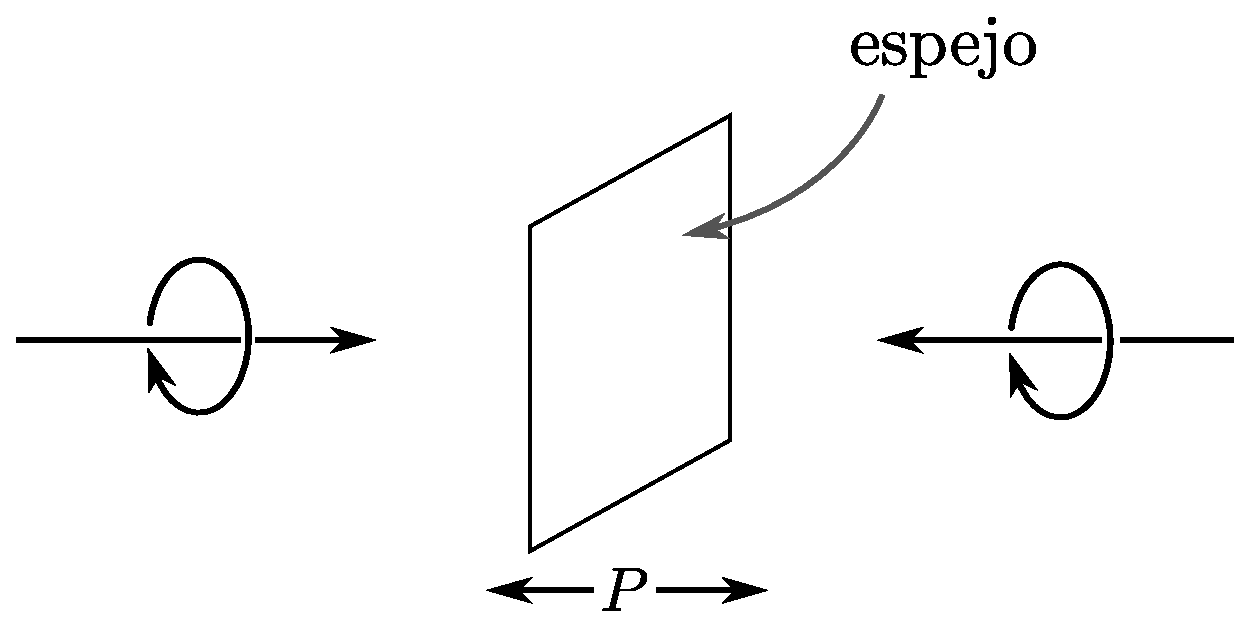
\includegraphics[scale=0.3]{Capitulos/Apendices/paridad.eps}
    \caption{La reflexión de un vector y un pseudovector apuntando perpendicularmente a un espejo ilustran una transformación de paridad en esa dirección.}
    \label{paridad}
\end{figure}

Sin embargo, podemos definir el campo de Dirac, de cuatro componentes complejas:
\begin{equation}
    \psi(x) = \mqty( \psi_{L}(x) \\ \psi_{R}(x) ),
\end{equation}
que bajo transformaciones de Lorentz (ortocronas propias) $x^{\mu} \mapsto x^{\prime \mu}=\Lambda^{\mu}_{~\nu}x^{\nu}$,
\begin{equation}
    \psi(x) \mapsto \psi^{\prime}(x^{\prime})=\Lambda_{D}\psi(x), \quad \Lambda_{D}= \smqty(\Lambda_{L} & 0 \\ 0 & \Lambda_{R}),
\end{equation}
y bajo paridad, $x^{\mu}=(t,\vb*{x}) \mapsto \tilde{x}^{\mu}=(t,-\vb*{x})$,
\begin{equation}
    \psi(x) \mapsto \psi^{\prime}(\tilde{x})=\mqty( \psi_{R}(\tilde{x}) \\ \psi_{L}(\tilde{x}) )=\mqty(0 & \vb*{1} \\ \vb*{1} & 0)\psi(\tilde{x}). 
\end{equation}

El conjugado de carga de un espinor de Dirac es otro espinor de Dirac,
\begin{equation}
    \psi^{c}=\mqty( \psi^{c}_{R}(x) \\ \psi^{c}_{L}(x) ) = \mqty( -\ii \sigma^{2}\psi_{R}^{*} \\ \ii \sigma^{2}\psi_{L}^{*})=-\ii \mqty( 0 & \sigma^2 \\ -\sigma^2 & 0 )\psi^{*}
\end{equation}

y, por supuesto , $\qty\big(\psi^{c})^{c} = \psi$. Además note que las coordenadas $x^{\mu}$ no cambian bajo conjugación de carga.\\

Los campos de Dirac y no los de Weyl son los objetos básicos en las teorías de campos invariantes bajo paridad, como la QED y la QCD.\\

Finalmente, un \emph{espinor de Majorana} es un espinor de Dirac en el que $\psi_L$ y $\psi_R$ no son independientes sino que

\begin{equation}
    \psi_R=\zeta \ii \sigma^2 \psi_L^* \quad \Rightarrow \quad \psi_M=\mqty(\psi_L \\ \zeta \ii \sigma^2 \psi_L^*), \quad  \abs{\zeta}^2=1.
\end{equation}

Tiene dos grados de libertad, como un espinor de Weyl, pero es autoconjugado de carga,

\begin{equation}
    \psi_M^c=\mqty(\zeta^* \psi_L \\ \ii \sigma^2 \psi_L^*) = \zeta^* \psi_M.
\end{equation}

\subsection{Campos vectoriales}

Bajo transformaciones de Lorentz, los campos vectoriales cumplen

\begin{equation}
    V^\mu(x) \mapsto V^{\prime \mu}\left(x^{\prime}\right)=\Lambda_\nu^\mu V^v(x) .
\end{equation}

Entonces, a partir de (\ref{eq_A103}) y (\ref{eq_A106}),

\begin{equation}
    \delta V^\mu(x)=\qty(\Lambda_{~\nu}^\mu-\delta_\nu^\mu) V^\nu(x)-\frac{\ii}{2} \omega_{\rho \sigma} L^{\rho \sigma} V^\mu(x) \equiv-\frac{\ii}{2} \omega_{\rho \sigma} J_V^{\rho \sigma} V^\mu(x) .
\end{equation}


Si escribimos, como antes, $J_V^{\rho \sigma}=L^{\rho \sigma}+S_V^{\rho \sigma}$, vemos que

\begin{equation}
    \Lambda_{~\nu}^\mu-\delta_{\nu}^\mu \equiv-\frac{\ii}{2} \omega_{\rho \sigma}\qty(S_V^{\rho \sigma})^{\mu}_{~\nu}=-\frac{\ii}{2} \omega_{\rho \sigma}\qty(J^{\rho \sigma})_{~\nu}^{\mu} \quad \Rightarrow \quad S_V^{\rho \sigma}=J^{\rho \sigma}.
\end{equation}

\section{Grupo de Poincare}

El grupo de Poincaré incluye las transformaciones de Lorentz y las traslaciones espacio-temporales,

\begin{equation}
    x^\mu \mapsto x^{\prime \mu}=x^\mu+a^\mu.
    \label{eq_A124}
\end{equation}

Si tomamos una traslación infinitesimal $a^\mu=\epsilon^\mu$,

\begin{IEEEeqnarray}{rCl}
    x^{\prime \mu} \equiv\qty(\vb*{1}-\mathrm{i} \epsilon_\rho P^\rho ) x^\mu & ~~\Rightarrow~~ & \delta x^\mu=\epsilon^\mu=-\mathrm{i} \epsilon_\rho P^\rho x^\mu \\
    & ~~\Rightarrow~~  & \quad P^\rho=\ii \partial^\rho .
\end{IEEEeqnarray}


Así que los generadores de las traslaciones son las 4 componentes del operador cuadrimomento $P^\mu$. La traslación (\ref{eq_A124}) se escribe, por tanto, $\exp (-\ii a_\mu P^\mu)$.\\

El álgebra de Poincaré, escrita en forma covariante, es

\begin{IEEEeqnarray}{rCl}
    \comm{P^\mu}{p^\nu} & = & 0, \\
    \comm{P^\mu}{J^{\rho \sigma}} & = & \ii \qty( g^{\mu \rho} P^\sigma-g^{\mu \sigma} P^\rho ),\\ \label{eq_A1.100}
    \comm{J^{\mu \nu}}{J^{\rho \sigma}} & = & \ii \qty(g^{\nu \rho}J^{\mu \sigma}  - g^{\mu \rho}J^{\nu \sigma}  - g^{\nu \sigma}J^{\mu \rho}  +g^{\mu \sigma}J^{\nu \rho} ).
\end{IEEEeqnarray}

La última línea corresponde al álgebra del subgrupo de Lorentz (\ref{eq_A106}). Las traslaciones son también un subgrupo. Conviene explicitar las relaciones de conmutación entre los generadores de las traslaciones y los de rotaciones y boosts:

\begin{IEEEeqnarray}{rCl}
    \comm{P^0}{J^k} & = & 0, \\
    \comm{P^k}{J^l} & = & \ii \epsilon^{klm} P^{m}, \\ 
    \comm{P^0}{K^k} & = & \ii P^k, \\
    \comm{P^k}{K^l} & = & \ii P^0 \delta^{kl}. 
\end{IEEEeqnarray}

Así que, como el hamiltoniano es $H = P^0$ (generador de las traslaciones temporales), tenemos que $\comm{H}{P^k}=\comm{H}{J^k}=0$ pero $\comm{H}{K^k} \neq 0$. Esto no significa que solo momento lineal y momento angular total son cantidades conservadas, porque $K^i$ depende explícitamente del tiempo de tal forma que

\begin{equation}
    \dv{x} K^k = \ii \comm{H}{K^k}+\pdv{t}K^k=0.
\end{equation}
Así que también hay cantidades conservadas asociadas a los boots, como se vió al estudiar el teorema de Noether en el siguiente tema.

\subsection{Representaciones sobre los campos}

Ya hemos visto que los campos forman representaciones de dimensión infinita del grupo de Lorentz, con generadores

\begin{equation}
    J^{\mu \nu}=L^{\mu \nu}+S^{\mu \nu},
    \label{eq_A1.107}
\end{equation}

donde $L^{\mu \nu}=\ii \qty(x^\mu \partial^\nu-x^\nu \partial^\mu )$ y $S^{\mu \nu}$ depende de si el campo es escalar, espinorial, etc. Hallemos ahora la representación de las traslaciones. Para ello, imponemos que para cualquier componente, ya sea tensorial o espinorial del campo, se cumple

\begin{equation}
    \phi^{\prime}\left(x^{\prime}\right)=\phi(x), \quad x^{\prime \mu}=x^\mu+a^\mu.
\end{equation}

Entonces, haciendo una translación infinitesimal $a^\mu=\epsilon^\mu$,

\begin{equation}
    \delta \phi(x) \equiv \phi^{\prime}(x) -  \phi (x) = \phi^{\prime}\left(x^{\prime}-\epsilon\right)-\phi(x)=\phi^{\prime}\left(x^{\prime}\right)-\epsilon^\mu \partial_\mu \phi(x)-\phi(x)=-\epsilon^\mu \partial_\mu \phi(x).
\end{equation}

Por tanto, comparando esta expresión con

\begin{equation}
    \phi^{\prime}\left(x^{\prime}-\epsilon\right)=\exp \left\{-\mathrm{i}\left(-\epsilon_\mu\right) P^\mu\right\} \phi^{\prime}\left(x^{\prime}\right) \Rightarrow \delta \phi(x)=\mathrm{i} \epsilon_\mu P^\mu \phi(x)
\end{equation}

tenemos que

\begin{equation}
    P^\mu=\ii \partial^\mu .
    \label{eq_A1.111}
\end{equation}

Para ver que lo que hemos obtenido es consistente, podemos comprobar la regla de conmutación (\ref{eq_A1.100}) usando la representación sobre campos de los generadores del grupo de Lorentz (\ref{eq_A1.107}) y de las traslaciones (\ref{eq_A1.111}) y teniendo en cuenta que $S^{\mu \nu}$ es independiente de las coordenadas espacio-temporales y por tanto conmuta con $\partial^\mu$,

\begin{IEEEeqnarray}{rCl}
    \comm{P^\mu}{J^{\rho \sigma}} = \comm{P^\mu}{L^{\rho \sigma}} &=& \left[\ii \partial^\mu, \ii \left(x^\rho \partial^\sigma-x^\sigma \partial^\rho\right)\right] \\
    &=&-\left(g^{\mu \rho} \partial^\sigma-g^{\mu \sigma} \partial^\rho \right)=\ii \left(g^{\mu \rho} P^\sigma-g^{\mu \sigma} P^\rho \right),
\end{IEEEeqnarray}

donde hemos aplicado la regla $\comm{A}{BC}=\comm{A}{B}C+A\comm{B}{C}$ y sustituido $\left[\partial^\mu, x^\nu\right]=g^{\mu \nu}$.

%-----------------
\subsection{Representaciones sobre estados de una partícula}

Ya hemos visto todo lo que necesitamos para construir lagrangianos de campos invariantes bajo Poincaré. Cuando se cuantizan los campos veremos que éstos crean y destruyen partículas (y antipartículas). Es conveniente entonces identificar el espacio de Hilbert de estados de una partícula, invariante bajo Poincaré, es decir, irreps del grupo de Poincaré etiquetadas por sus operadores de Casimir y cuyos vectores vienen especificados por números cuánticos que son autovalores de un conjunto de generadores que conmuten entre sí (y de otros operadores que conmuten con ellos), $\ket{\vb*{p},j_{3},\ldots}$.\\

El grupo de Poincaré tiene dos operadores de Casimir:

\begin{equation}
    m^2=P_\mu P^\mu \quad \mathrm{y} \quad W_\mu W^\mu,
\end{equation}

donde $W^\mu$ es el cuadrivector de \emph{Pauli-Lubanski} definido por
\begin{equation}
   W^\mu=-\frac{1}{2} \epsilon^{\mu \nu \rho \sigma} J_{\nu \rho} P_\sigma . 
\end{equation}

Ambos operadores conmutan, pues

\begin{IEEEeqnarray}{rCl}
    \comm{W^\mu}{P^\alpha} & = & -\frac{1}{2} \epsilon^{\mu \nu \rho \sigma}\comm{J_{\nu \rho} P_\sigma}{P^\alpha}\\
    &=&-\frac{1}{2} \epsilon^{\mu \nu \rho \sigma}\left(J_{v \rho}\comm{P_\sigma}{P^\alpha} +\comm{J_{v \rho}}{ P^\alpha}P_\sigma\right) \\
    &=&-\frac{\ii}{2} \epsilon^{\mu \nu \rho \sigma}\left(g_\rho^\alpha P_\nu-g_\nu^\alpha P_\rho\right) \\
    &=&-\frac{\ii}{2} \epsilon^{\mu v \alpha \sigma} P_v+\frac{\ii}{2} \epsilon^{\mu \alpha \rho \sigma} P_\rho=0 .
\end{IEEEeqnarray}

Además $m^2=P_\mu P^\mu$ y $W_\mu W^\mu$ son invariantes Lorentz. Por tanto, son operadores de Casimir (conmutan con $P^\rho$ y $J^{\rho \sigma}$ ) y podemos usar sus autovalores para etiquetar las irreps y calcularlos en el sistema de referencia que queramos. Tenemos que distinguir dos casos:

\begin{itemize}
    \item Caso $m \neq 0$ \\
    
    Usemos el sistema de referencia en reposo, $p^\mu=(m, 0,0,0)$. Entonces,

    \begin{equation}
        \left.\begin{array}{l}
        W^0=0 \\
        W^i=-\frac{m}{2} \epsilon^{i j k 0} J^{j k}=\frac{m}{2} \epsilon^{i j k} J^{j k}=m J^i
        \end{array}\right\} \quad \Rightarrow \quad W_\mu W^\mu=-m^2 j(j+1) .
    \end{equation}
    Es decir, las irreps están etiquetadas por $m, j$ y los vectores por $\ket{j_3=-j \ldots j}$, donde $j$ es el espín. Vemos que las partículas masivas de espín $j$ tienen $2 j+1$ grados de libertad. Esto es así porque, una vez que se ha hecho un boost para llevar la partícula masiva al sistema de referencia en el que su cuadrimomento es $p^\mu=(m, 0,0,0)$, tenemos total libertad para rotar en tres dimensiones el sistema. Decimos que el grupo $\SU2$ es su grupo de Lorentz pequeño (conjunto de transformaciones de Lorentz que dejan invariante una elección dada de $p^\mu$).
    \vspace{0.5cm}

    \item Caso $m=0$\\
    
    No existe el sistema de referencia en reposo. Podemos elegir uno en el que $p^\mu=(\omega, 0,0, \omega)$, que describe una partícula sin masa que se mueve en la dirección del eje $z$. Entonces,

    \begin{equation}
        \left.\begin{array}{rl}
        -W^0 & =W^3=\omega J^3 \\
        W^1 & =\omega\left(J^1+K^2\right) \\
        W^2 & =\omega\left(J^2-K^1\right)
        \end{array}\right\} 
        \quad \Rightarrow \quad W_\mu W^\mu=-\omega^2\left[\left(J^1+K^2\right)^2+\left(J^2-K^1\right)^2\right].
    \end{equation}
    En este caso el grupo pequeño son las rotaciones en el plano perpendicular a la dirección del movimiento (el plano $(x, y)$ en nuestra elección), que es $\SO2$, cuyas irreps son unidimensionales (grupo abeliano) y se etiquetan por un número $h \in\left\{0, \pm \frac{1}{2}, \pm 1, \ldots\right\}$ llamado helicidad (proyección del momento angular en la dirección del movimiento):\footnote{Los elementos de $\SO2$ en la irrep $h$ vienen dados por $R(\theta) = \exp \qty( - \ii h\theta)$.}

    \begin{equation}
        h=\hat{\vb*{p}} \cdot \vb*{J}.
    \end{equation}
    
    Nótese que $h=j_3$ en nuestra elección de dirección del movimiento, con $j_3=\pm j$. Las irreps $h$ y $-h$ son distintas (no se mezclan bajo transformaciones de Poincaré), aunque en las teorías simétricas bajo paridad las partículas sin masa correspondientes reciben el mismo nombre y se dice que están en dos estados distintos de helicidad. Así se habla de fotón ( $m=0, j=1$ ) dextrógiro/levógiro si $h=\pm 1$. También decimos que el fotón es una partícula sin masa de espín $1$, aunque en realidad no existe el estado con $j_3=0$. Del mismo modo, veremos que los campos de Weyl sin masa $\psi_L$ y $\psi_R$ $\left(m=0, j=\frac{1}{2}\right)$ tienen helicidad $h=-\frac{1}{2}$, $h=+\frac{1}{2}$, respectivamente y representan a partículas distintas si la teoría no es simétrica bajo paridad (e.g. en el modelo estándar si los neutrinos no tienen masa el neutrino es $\nu_L$ y el $\nu_R$ podría no existir).
    
    Un último comentario: siempre podemos hablar de helicidad como la proyección del momento angular en la dirección del movimiento, pero solamente es una cantidad invariante bajo transformaciones de Poincaré para partículas sin masa. A veces se usa el término quiralidad, que tiene que ver con si la partícula se transforma bajo la representación del espinor izquierdo o del espinor derecho del grupo de Lorentz. La quiralidad coincide con la helicidad para partículas sin masa.
\end{itemize}

\begin{cabox}
    \textbf{Aspectos para llevarse de esta sección}
    \renewcommand{\labelitemi}{\ding{42}}
    \begin{itemize}
        \item Grupos para recordar: grupo de Lorentz y subgrupos, grupo de Poincaré.
        \item $so(3,1)=su(2)+su(2) \Longrightarrow$ Irreps de $\mathrm{SO}(3,1)$ se etiquetan por $\left(j_1, j_2\right)$ (espín de cada $su(2)$).
        \item Un espinor es un elemento sobre el cual actúa la irrep de $s u(2)$ de $j=1/2$.
        \item Espinor de Weyl 
              $\begin{cases}
              \text{izquierdo} \rightarrow\left(\frac{1}{2}, 0\right)\\ 
              \text{derecho} \rightarrow \left(0, \frac{1}{2}\right) 
              \end{cases}$
        \item Las irreps del grupo de Poincaré van a estar asociadas al concepto de partícula elemental en nuestra teoría.
    \end{itemize}
\end{cabox}



%-----------------------------------------------      Fin Capítulo 1 -------------------------------------------------------------------------------------------